\documentclass[11pt,a4paper,oneside,openany]{book}
\usepackage[margin=25mm,headheight=15pt]{geometry}
\usepackage[T1]{fontenc}
\usepackage[utf8]{inputenc}
\usepackage{lmodern,microtype}
\usepackage{amsmath,amssymb,mathtools,bm}
\usepackage{graphicx,xcolor,booktabs,longtable,array}
\usepackage{siunitx,enumitem,listings}
\usepackage{tikz}
\usetikzlibrary{arrows.meta,calc,positioning}
\usepackage{fancyhdr}
\usepackage{hyperref}
\hypersetup{colorlinks=true,linkcolor=blue!45!black,citecolor=green!35!black,urlcolor=blue!55!black,pdftitle={Optical Aberrations: Orders, Derivations, and Design},pdfauthor={Self-study optics series}}
\setlength{\emergencystretch}{3em}
\setlength{\parskip}{0.35em}
\setcounter{tocdepth}{1}
\setcounter{secnumdepth}{2}
\setlist{itemsep=0.25em,topsep=0.4em}
\pagestyle{fancy}
\fancyhf{}
\fancyhead[L]{\small\nouppercase{\leftmark}}
\fancyfoot[C]{\thepage}
\renewcommand{\chaptermark}[1]{\markboth{\thechapter.\ #1}{}}
\lstset{basicstyle=\ttfamily\footnotesize,breaklines=true,columns=fullflexible,keepspaces=true,frame=single,rulecolor=\color{black!20},showstringspaces=false,tabsize=4}
\begin{document}
\frontmatter
\hypersetup{pageanchor=false}
\begin{titlepage}
\centering
\vspace*{18mm}
{\large SELF-STUDY OPTICS SERIES\par}
\vspace{17mm}
{\Huge\bfseries Optical Aberrations\par}
\vspace{6mm}
{\LARGE Orders, Derivations, and Design\par}
\vspace{13mm}
{\Large A first-principles course for mirrors and lenses\par}
\vspace{18mm}
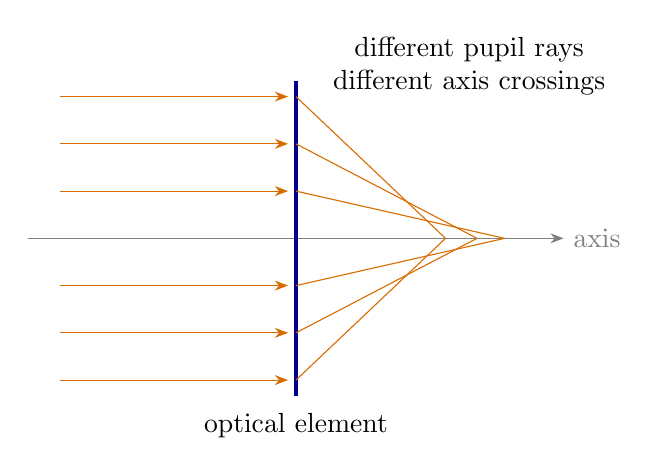
\begin{tikzpicture}[x=1cm,y=1cm,>=Stealth]
\draw[gray,->] (-3.4,0)--(3.4,0) node[right] {axis};
\draw[very thick,blue!55!black] (0,-2)--(0,2);
\foreach \h/\f in {1.8/1.9,1.2/2.3,0.6/2.65,-0.6/2.65,-1.2/2.3,-1.8/1.9}{
\draw[orange!85!black,->] (-3,\h)--(-0.1,\h);
\draw[orange!85!black] (0,\h)--(\f,0);
}
\node[below] at (0,-2.1) {optical element};
\node[above,align=center] at (2.2,1.7) {different pupil rays\\different axis crossings};
\end{tikzpicture}
\vfill
{\large Primary and higher-order theory, explicit calculations,\par mirror and lens examples, and exercises with solutions\par}
\vspace{8mm}
{10 September 2026\par}
\end{titlepage}
\hypersetup{pageanchor=true}
\setcounter{page}{1}
\chapter*{How to study this book}
\addcontentsline{toc}{chapter}{How to study this book}
An aberration is a departure from a specified ideal image or wavefront. To calculate one, you must first define the ideal. This book begins with how rays travel and how a simple lens or mirror forms an image. It then derives the departures systematically, including how the departures change with pupil position and object field.

Part I is a self-contained introduction for a reader who has never studied optics. It includes the mathematical operations used later. Part II derives primary aberrations, constructs the higher-order hierarchy, and relates these mathematical descriptions to physical mirror and lens designs. The emphasis is on reasoning you can reproduce: coordinate definitions, optical path expansions, gradients, numerical estimates, and checks against exact geometry.

\paragraph{Three meanings of order.}
Keep three questions separate throughout your study: what is the total degree of the wavefront polynomial in pupil and field coordinates; what is the degree of the transverse ray error; and what is the radial index of a Zernike polynomial? A term can be called third order in one description and fourth order in another. The chapters derive the connection and explain where a leading paraxial conversion ceases to be sufficient.

\paragraph{Suggested progression.}
Study the foundations first, then derive each primary aberration and draw its ray fan. Reproduce the spherical mirror example by hand before running the computational check. Next work through the invariant construction for higher orders, the lens examples, chromatic effects, and the design exercises. Keep a notebook recording every reference plane, aperture, sign convention, and approximation. An unexplained factor of two is an invitation to reconstruct the optical path, not to memorize another rule.

\paragraph{Companion material.}
The book in \texttt{../Zernike Constants/} develops disk orthogonality and wavefront fitting in greater depth. Both books repeat the introductory foundations for independent use. The shared \texttt{../verify\_optics.py} script provides reproducible checks of modal normalization and exact rays; its saved results are in \texttt{../numerical\_checks.txt}. All prescriptions used for numerical examples are explicit teaching examples, not measured data from an instrument.

\paragraph{Scope and next steps.}
This is a bridge into research, including reproducible modelling and interpretation of numerical results. It does not replace a complete treatment of Hamiltonian optics, general surface-by-surface high-order aberration sums, polarization-sensitive diffraction, or a validated industrial design code. It teaches when the approximations work and how an exact ray trace can expose their failure. Further reading is listed at the end.

\chapter*{Notation and convention card}
\addcontentsline{toc}{chapter}{Notation and convention card}
Keep this page beside your calculations. Individual examples may introduce local symbols, but each defines its geometry before using it.

\renewcommand{\arraystretch}{1.05}
\begin{longtable}{@{}>{\raggedright\arraybackslash}p{0.17\linewidth}>{\raggedright\arraybackslash}p{0.46\linewidth}>{\raggedright\arraybackslash}p{0.29\linewidth}@{}}
\toprule
Symbol & Meaning & Typical units or range \\
\midrule
\endhead
$\lambda_0$ & Vacuum wavelength & nm, $\mu$m, or mm; convert consistently \\
$n,n',n_g$ & Refractive indices in incident, output, and glass regions & Dimensionless \\
$\mathcal{L}$ & Optical path length $\int n\,\mathrm{d}\ell$ & Length \\
$S$ & Eikonal; phase expressed as optical length & Length \\
$W$ & Actual minus ideal eikonal at the stated comparison points & Length; waves only when explicitly divided by $\lambda_0$ \\
$\phi$ & Optical phase, $2\pi S/\lambda_0$ & Radians \\
$\bm{d},\bm{N}$ & Unit ray direction and unit surface normal & Dimensionless vectors \\
$R,c=1/R$ & Vertex radius and curvature & Length and inverse length \\
$K$ & Conic constant in the specified sag equation & Dimensionless \\
$a,r$ & Physical pupil radius and physical radial coordinate & Length \\
$\rho,\theta$ & Normalized radius $r/a$ and pupil azimuth & $0\leq\rho\leq1$; radians \\
$u,v$ & Often normalized Cartesian pupil coordinates in wavefront sections & Dimensionless; local definitions take precedence \\
$u,p=nu$ & In first-order ray matrices, small angle and reduced angle & Radians and index times radians \\
$H$ & Normalized field magnitude in invariant expansions & Dimensionless when normalized \\
$f,L$ & Focal length; distance from comparison plane to reference focus & Length; generally different \\
$Z_n^m$ & Real RMS-normalized disk mode & Dimensionless; here $n$ is a radial integer, not an index of refraction \\
$c_n^m$ & Coefficient multiplying $Z_n^m$ in a wavefront expansion & Same units as $W$ \\
$\langle\cdot\rangle$ & Specified pupil average; uniform area by default & Preserves the units of its argument \\
$\sigma_W$ & RMS wavefront deviation after the stated removals & Length \\
$\Delta\bm{x}$ & Actual minus ideal transverse ray intercept & Length \\
\bottomrule
\end{longtable}
\renewcommand{\arraystretch}{1}
\clearpage

\paragraph{Geometry and OPD.}
For a transmitting system the local forward axis is normally $+z$. A signed spherical radius is positive when its centre of curvature is downstream. Mirror examples explicitly specify the direction before and after reflection. Our OPD sign is $W=S_{\rm actual}-S_{\rm ideal}$, giving the leading forward image-space relation $\Delta\bm{x}\simeq(L/n')\nabla_\perp W$. Changing the definition of OPD reverses the corresponding signed coefficients.

\paragraph{Modes and pupil.}
Unless explicitly stated otherwise, Zernike functions are real, orthonormal under the full-disk area average, with $m>0$ for $\cos(m\theta)$ and $m<0$ for $\sin(|m|\theta)$. A pair $(n,m)$ identifies a function; a single number requires a named ordering convention. Coefficients depend on the pupil radius, coordinate surface, obscurations or weights, reference sphere, and removed modes.

\paragraph{Order and meaning.}
A wavefront polynomial's total degree in pupil and field variables, the degree of its transverse ray error, and the radial index of a Zernike mode answer different questions. Terms called ``spherical'' or ``coma'' in a Zernike fit include lower powers needed for orthogonality. They are not simply the corresponding highest monomials. Surface Zernike amplitudes are not wavefront amplitudes until the reflection or refraction conversion and pupil mapping have been applied.

\tableofcontents
\mainmatter
\part{Foundations: from light to an optical model}
% This foundation is repeated in both volumes for independent study.
\chapter{The mathematical language of optics}
\label{fnd:math}

\section{What an optical model describes}
Imagine a small luminous point, a lens, and a sheet of paper. Light leaving the point travels in many directions. Some of those directions reach the lens. A successful imaging system redirects that light into a small region on the paper. A mirror accomplishes redirection by reflection; a lens does it by refraction. An optical design specifies the surfaces, their positions, the materials between them, and which rays are admitted.

There are two complementary descriptions. A \emph{ray} describes a local direction of energy propagation in the geometrical approximation. A \emph{wavefront} describes equal phase. Rays let us calculate intersections and image positions. Wavefronts tell us whether light arriving by different paths adds constructively. An aberration can therefore be described by misplaced rays or by an error in optical phase. The two descriptions are connected but their numerical measures have different units.

Before deriving an equation, write down what its variables represent. A surface height, a ray height, and an optical path difference may all be measured in millimetres; they are nevertheless different quantities. Similarly, a physical pupil radius and a normalized radius may have the same numerical value in one example but different dimensions.

\section{Units, angles, and dimensionless coordinates}
We use the vacuum wavelength $\lambda_0$. The units most often encountered are
\[
1\ \mathrm{mm}=10^{-3}\ \mathrm{m},\qquad
1\ \mu\mathrm{m}=10^{-6}\ \mathrm{m},\qquad
1\ \mathrm{nm}=10^{-9}\ \mathrm{m}.
\]
Thus $633\ \mathrm{nm}=0.000633\ \mathrm{mm}$. If an optical path error is $W=31.65\ \mathrm{nm}$, its value in waves at this wavelength is $W/\lambda_0=0.05$. The phase error is $2\pi W/\lambda_0=0.31416$ radians. At $13.5\ \mathrm{nm}$ the same path error is about $2.344$ waves. A surface acceptable at one wavelength may be unacceptable at another even when the ray geometry is identical.

An angle in radians is arc length divided by radius. One full revolution is $2\pi$ radians, so $1^\circ=\pi/180$ radians. Series such as $\sin u\simeq u$ assume radians. Substituting $u=5$ for five degrees would be a serious error; the correct number is approximately $0.08727$.

For a circular pupil of physical radius $a$, define
\begin{equation}
x=a\rho\cos\theta,\qquad y=a\rho\sin\theta,
\qquad 0\leq\rho\leq1,\quad 0\leq\theta<2\pi.
\label{fnd:pupilcoords}
\end{equation}
Here $x,y,a$ have units of length and $\rho$ is dimensionless. The angle $\theta$ increases counterclockwise from the positive $x$ axis toward the positive $y$ axis when looking at the plotted pupil. State the physical viewing direction separately when comparing two instruments, because looking from the opposite side reverses handedness.

\section{Functions, slopes, and curvature}
A function assigns an output to an input. A sag function $z=s(x,y)$ gives a surface's axial position at transverse point $(x,y)$. For a rotationally symmetric surface, $s$ depends only on $r=\sqrt{x^2+y^2}$.

The derivative is a limiting slope:
\[
\frac{\mathrm{d}s}{\mathrm{d}r}
=\lim_{\Delta r\to0}\frac{s(r+\Delta r)-s(r)}{\Delta r}.
\]
For $s(r)=cr^2/2$, expand $(r+\Delta r)^2$, subtract $r^2$, and divide by $\Delta r$ to get $cr+c\Delta r/2$. Taking the limit gives $s'(r)=cr$. The second derivative $s''(r)=c$ describes how fast the slope changes. For a shallow spherical surface, $c=1/R$ is its vertex curvature.

A partial derivative varies one coordinate while holding the other fixed. The transverse gradient is
\[
\nabla_\perp W=
\left(\frac{\partial W}{\partial x},\frac{\partial W}{\partial y}\right).
\]
For $W=A(x^2+y^2)^2$,
\[
\frac{\partial W}{\partial x}=4Ax(x^2+y^2),\qquad
\frac{\partial W}{\partial y}=4Ay(x^2+y^2).
\]
The coefficient $A$ here has units of inverse length cubed if $W$ is a length. If instead $W=B\rho^4$, then $B$ has units of length. The two coefficients satisfy $B=Aa^4$. Confusing them gives errors that grow as the fourth power of the aperture radius.

The chain rule handles normalization. With $u=x/a$ and $v=y/a$,
\[
\frac{\partial W}{\partial x}
=\frac{1}{a}\frac{\partial W}{\partial u}.
\]
The factor $1/a$ is essential when converting a fitted wavefront into a physical ray angle.

\section{Integrals and the area measure on a disk}
An integral adds infinitesimal contributions. The one-dimensional identity
\[
\int_0^1\rho^q\,\mathrm{d}\rho=\frac{1}{q+1}\qquad(q>-1)
\]
follows because the derivative of $\rho^{q+1}/(q+1)$ is $\rho^q$.

A small polar patch has radial width $\mathrm{d}r$ and tangential width $r\,\mathrm{d}\theta$. Its area is therefore $r\,\mathrm{d}r\,\mathrm{d}\theta$. After setting $r=a\rho$,
\[
\mathrm{d}A=a^2\rho\,\mathrm{d}\rho\,\mathrm{d}\theta.
\]
The area of the disk follows immediately: $a^2\int_0^{2\pi}\int_0^1\rho\,\mathrm{d}\rho\,\mathrm{d}\theta=\pi a^2$. The area average of a function is thus
\begin{equation}
\langle F\rangle=
\frac{1}{\pi}\int_0^{2\pi}\int_0^1
F(\rho,\theta)\rho\,\mathrm{d}\rho\,\mathrm{d}\theta.
\label{fnd:average}
\end{equation}
In particular,
\[
\langle\rho^q\rangle=\frac{2}{q+2},\qquad
\langle\rho^2\rangle=\frac12,\quad
\langle\rho^4\rangle=\frac13,\quad
\langle\rho^6\rangle=\frac14.
\]
These simple moments will repeatedly replace lengthy integrations.

The mean-subtracted root-mean-square value of a wavefront is
\begin{equation}
\sigma_W=\sqrt{\langle(W-\langle W\rangle)^2\rangle}
=\sqrt{\langle W^2\rangle-\langle W\rangle^2}.
\label{fnd:rms}
\end{equation}
To obtain the second equality, expand the square, use linearity of the integral, and recognize that $\langle W\rangle$ is a constant. For $W=B\rho^2$, the mean is $B/2$ and the variance is $B^2(1/3-1/4)=B^2/12$, giving $\sigma_W=|B|/\sqrt{12}$. The peak-to-valley error is $|B|$, a different statistic.

\section{Taylor expansions and what an omitted term means}
Near $\epsilon=0$, the binomial expansion gives
\begin{align}
(1+\epsilon)^{1/2}
&=1+\frac{\epsilon}{2}-\frac{\epsilon^2}{8}
+\frac{\epsilon^3}{16}-\frac{5\epsilon^4}{128}+
O(\epsilon^5),\\
(1-\epsilon)^{1/2}
&=1-\frac{\epsilon}{2}-\frac{\epsilon^2}{8}
-\frac{\epsilon^3}{16}-\frac{5\epsilon^4}{128}+
O(\epsilon^5).
\end{align}
The notation $O(\epsilon^5)$ means that the neglected remainder scales no faster than a constant times $|\epsilon|^5$ sufficiently near zero. It is not an error estimate valid at arbitrary aperture. To use an expansion reliably, identify its dimensionless small quantity and check convergence at the largest ray height of interest.

For example,
\begin{align}
\sqrt{L^2+r^2}
&=L\sqrt{1+r^2/L^2}\\
&=L+\frac{r^2}{2L}-\frac{r^4}{8L^3}
+\frac{r^6}{16L^5}+O(r^8/L^7),\qquad L>0.
\label{fnd:distance-series}
\end{align}
Every term has dimensions of length. The expansion parameter is $(r/L)^2$. For $r/L=0.05$, the quartic correction is smaller than the quadratic term by $(r/L)^2/4=0.000625$. That may be tiny geometrically but still many nanometres of optical path, which can matter in a short-wavelength instrument.

For a sphere with positive radius $R$ and vertex at $z=0$,
\begin{align}
s(r)&=R-\sqrt{R^2-r^2}\\
&=\frac{r^2}{2R}+\frac{r^4}{8R^3}
+\frac{r^6}{16R^5}+\frac{5r^8}{128R^7}+\cdots.
\label{fnd:sphere-sag}
\end{align}
The first term is a parabola in a meridional section. A sphere and a paraboloid can therefore have the same vertex curvature while differing away from the axis. Those apparently small higher-power differences are a central source of aberration.

\section{Vectors and a minimal introduction to matrices}
A three-dimensional vector $\bm{r}=(x,y,z)$ describes position or displacement. Its length is $|\bm{r}|=\sqrt{x^2+y^2+z^2}$. The dot product
\[
\bm{a}\cdot\bm{b}=a_xb_x+a_yb_y+a_zb_z
=|\bm{a}|\,|\bm{b}|\cos\gamma
\]
measures the component of one vector along the other; $\gamma$ is their included angle. A unit vector has length one. A straight ray is $\bm{r}(t)=\bm{r}_0+t\bm{d}$, with unit direction $\bm{d}$ and distance parameter $t$ in units of length.

A matrix encodes a linear operation. For example,
\[
\begin{pmatrix}A&B\\C&D\end{pmatrix}
\begin{pmatrix}y\\p\end{pmatrix}
=\begin{pmatrix}Ay+Bp\\Cy+Dp\end{pmatrix}.
\]
If operation $M_1$ acts first and $M_2$ acts second, the combined result is $M_2M_1\bm{v}$. The rightmost matrix acts first. Changing that order usually changes the answer because refraction followed by translation is physically different from translation followed by refraction.

\chapter{Why light reflects, refracts, and accumulates phase}
\label{fnd:light}
\section{The domain of ray optics}
Light is an electromagnetic wave. In a simple isotropic transparent medium the refractive index $n$ relates the phase speed to the vacuum speed by $v=c/n$. In this introductory model, $n$ is real and may depend on wavelength. Absorption and multilayer reflection require a complex optical response, discussed later where relevant.

Ray optics is a short-wavelength approximation: the relevant surface and field variations are smooth on the wavelength scale, and diffraction is not needed to locate the leading geometrical paths. The condition is not merely that a lens is bigger than a wavelength. A small sharp feature, an aperture edge, a caustic, or a narrow focal region can require a wave treatment even in a large apparatus. We use rays for the path geometry and wavefront phase for the first connection to image quality.

\section{Optical path length and phase}
If light travels a small geometric distance $\mathrm{d}\ell$ in index $n$, it accumulates phase $2\pi n\,\mathrm{d}\ell/\lambda_0$. Summing along a path gives
\begin{equation}
\mathcal{L}=\int n\,\mathrm{d}\ell,
\qquad \phi=\frac{2\pi}{\lambda_0}\mathcal{L}+\phi_{\rm initial}.
\label{fnd:opl}
\end{equation}
The quantity $\mathcal{L}$ is optical path length (OPL), not geometrical distance. In homogeneous segments it reduces to $\mathcal{L}=\sum_j n_j\ell_j$.

For $10\ \mathrm{mm}$ in air approximated by $n=1$ followed by $5\ \mathrm{mm}$ of index $1.5$, the geometrical length is $15\ \mathrm{mm}$ but the OPL is $17.5\ \mathrm{mm}$. Replacing $5\ \mathrm{mm}$ of air by that glass increases OPL by $2.5\ \mathrm{mm}$. Optical phase is controlled by that difference, not by the total thickness alone.

For two coherent scalar fields of real amplitudes $A_1,A_2$, the intensity after superposition is proportional to
\[
|A_1e^{i\phi_1}+A_2e^{i\phi_2}|^2
=A_1^2+A_2^2+2A_1A_2\cos(\phi_1-\phi_2).
\]
This identity follows by multiplying the complex sum by its complex conjugate. Equal phases reinforce; a phase difference of $\pi$ can cancel equal amplitudes. A geometrically small path mismatch can therefore have a large effect on image intensity.

\section{Fermat's principle: stationary optical path}
Fermat's principle states that the physical ray makes the optical path stationary under small allowed changes of path with endpoints held fixed. \emph{Stationary} means that the first-order change vanishes. The path need not be a global minimum.

Derive Snell's law in a two-dimensional plane. Place a flat interface at $z=0$, with source $A=(x_A,-h_1)$ in index $n_1$ and destination $B=(x_B,h_2)$ in index $n_2$. Let the unknown crossing point be $P=(x,0)$. The optical path is
\[
\mathcal{L}(x)=n_1\sqrt{(x-x_A)^2+h_1^2}
+n_2\sqrt{(x_B-x)^2+h_2^2}.
\]
Differentiation gives
\[
\frac{\mathrm{d}\mathcal{L}}{\mathrm{d}x}
=n_1\frac{x-x_A}{\sqrt{(x-x_A)^2+h_1^2}}
-n_2\frac{x_B-x}{\sqrt{(x_B-x)^2+h_2^2}}.
\]
Each ratio is the sine of the corresponding signed angle to the interface normal. Setting the derivative to zero yields
\begin{equation}
n_1\sin i=n_2\sin t.
\label{fnd:snell}
\end{equation}
If $n_2>n_1$ and the incident angle is positive, then $t<i$: the ray bends toward the normal. At normal incidence both angles vanish and the direction does not change, although phase accumulation does.

For reflection, put both endpoints on the same side of the interface and use the same index for both path segments. The analogous derivative sets the two signed tangential projections equal. The normal component reverses, yielding equality of incident and reflected angles measured from the normal. An ideal plane mirror redirects a converging or diverging bundle without acquiring optical power in its own local plane.

\begin{figure}[htbp]
\centering
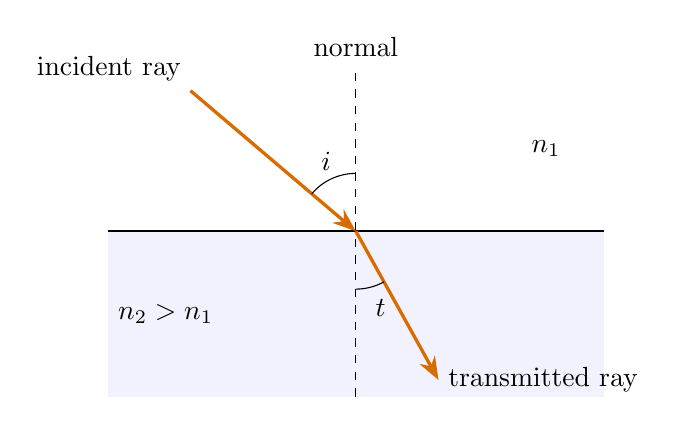
\begin{tikzpicture}[scale=1.05,>=Stealth]
\fill[blue!5] (-3,-2) rectangle (3,0);
\draw[thick] (-3,0)--(3,0);
\draw[dashed] (0,-2)--(0,2);
\draw[very thick,orange!85!black,->] (-2,1.7)--(0,0);
\draw[very thick,orange!85!black,->] (0,0)--(1,-1.8);
\node[above left] at (-2,1.7) {incident ray};
\node[right] at (1,-1.8) {transmitted ray};
\node at (2.3,1) {$n_1$};
\node at (-2.3,-1) {$n_2>n_1$};
\node[above] at (0,2) {normal};
\draw (0,0.7) arc[start angle=90,end angle=139.6,radius=0.7];
\node at (-0.36,0.85) {$i$};
\draw (0,-0.7) arc[start angle=-90,end angle=-60.9,radius=0.7];
\node at (0.30,-0.93) {$t$};
\end{tikzpicture}
\caption{Angles in Snell's law are measured from the normal, not from the interface. Geometry is schematic.}
\end{figure}

\section{Exact vector reflection}
Let $\bm{d}$ be the incident unit direction and $\bm{N}$ any unit normal to the reflecting surface. Split $\bm{d}$ into normal and tangent components:
\[
\bm{d}_\perp=(\bm{d}\cdot\bm{N})\bm{N},\qquad
\bm{d}_\parallel=\bm{d}-\bm{d}_\perp.
\]
Specular reflection preserves the tangent component and reverses the normal component. Therefore
\begin{equation}
\boxed{\bm{d}_{\rm r}=\bm{d}-2(\bm{d}\cdot\bm{N})\bm{N}.}
\label{fnd:reflection}
\end{equation}
Replacing $\bm{N}$ by $-\bm{N}$ does not change this expression. With $\bm{d}=(0,0,-1)$ and $\bm{N}=(0,0,1)$, reflection gives $(0,0,1)$ as expected. Reflection at a perfect plane changes direction; a spatially constant coating phase does not change the outgoing wavefront error after piston removal.

\section{Exact vector refraction and total internal reflection}
For refraction choose $\bm{N}$ to point into the incident medium, so $\bm{d}\cdot\bm{N}<0$. Set
\[
\eta=\frac{n_1}{n_2},\qquad c_i=-\bm{d}\cdot\bm{N}.
\]
The incident tangent component is $\bm{d}+c_i\bm{N}$. Snell's law scales it by $\eta$, while normalization fixes the transmitted normal component. Thus
\begin{align}
c_t&=\sqrt{1-\eta^2(1-c_i^2)},\\
\bm{d}_{\rm t}&=\boxed{\eta\bm{d}+(\eta c_i-c_t)\bm{N}.}
\label{fnd:vector-snell}
\end{align}
The negative normal component $-c_t\bm{N}$ sends the ray into the second medium. Verify normal incidence: $\bm{d}=-\bm{N}$ gives $\bm{d}_{\rm t}=-\bm{N}$.

If the expression under the square root is negative, there is no propagating transmitted ray in this geometrical model. This is total internal reflection. For $n_1>n_2$, its threshold is $\sin i_c=n_2/n_1$. A glass-to-air interface with $n_1=1.5$ has $i_c\simeq41.81^\circ$. This is a propagation condition, not a statement that polarization-dependent phase can be neglected during reflection.

\section{Eikonal, wavefront normals, and the ray limit}
Write a monochromatic scalar field locally as
\[
U(\bm{r})=A(\bm{r})e^{ik_0S(\bm{r})},\qquad k_0=2\pi/\lambda_0.
\]
Here $S$ has units of length and is called the eikonal. The suppressed time dependence is $e^{-i\omega t}$, so increasing spatial phase corresponds to propagation along $\nabla S$. Substitute this form into the scalar Helmholtz equation $\nabla^2U+k_0^2n^2U=0$. Applying the product rule twice and cancelling the exponential gives
\[
\nabla^2A+2ik_0\nabla A\cdot\nabla S
+ik_0A\nabla^2S-k_0^2A|\nabla S|^2+k_0^2n^2A=0.
\]
In the short-wavelength limit the terms proportional to $k_0^2$ dominate if the amplitude and material vary slowly. Their cancellation requires
\begin{equation}
|\nabla S|^2=n^2,\qquad \bm{d}=\frac{\nabla S}{n}.
\label{fnd:eikonal}
\end{equation}
A wavefront is a level surface $S=\mathrm{constant}$, so its normal is $\nabla S$. This explains the statement that rays are normal to wavefronts in an isotropic medium. At a caustic, several ray branches can reach the same point; a single smooth eikonal then requires branchwise interpretation. The full electromagnetic problem also contains vector and polarization effects absent from this scalar derivation.

\chapter{First-order images: mirrors, lenses, and ray matrices}
\label{fnd:imaging}
\section{Coordinates and the paraxial approximation}
For transmitted systems, take the optical axis along $+z$, let ray height in a meridional section be $y$, and let $u$ be its small signed angle to $+z$. The paraxial approximation uses
\[
\sin u\simeq u,\qquad \tan u\simeq u,\qquad \cos u\simeq1.
\]
It retains only terms linear in ray heights and angles. It predicts ideal first-order imaging but discards the nonlinear terms that cause geometrical aberrations. ``Paraxial'' is an approximation to a physical ray, not a separate type of light.

A radius of curvature is positive if the centre of curvature lies downstream of its vertex. Thus the first surface of a usual biconvex lens has $R_1>0$ and the second has $R_2<0$. For a mirror we state the incident and reflected axes explicitly; blindly carrying the transmitted-system signs through a reversal of propagation is a frequent source of mistakes.

\section{Paraxial power of one refracting surface}
Near a vertex, $s(y)\simeq y^2/(2R)$ and the slope is $y/R$. A normal oriented approximately along $+z$ has small angle $\alpha\simeq-y/R$ to the axis. The signed incident and refracted angles relative to that normal are $u-\alpha$ and $u'-\alpha$. Linearizing Snell's law gives
\[
n(u-\alpha)=n'(u'-\alpha).
\]
Rearrange and substitute $\alpha=-y/R$:
\begin{equation}
n'u'=nu-\frac{n'-n}{R}y.
\label{fnd:surface-power}
\end{equation}
Define reduced angle $p=nu$ and surface power $\Phi=(n'-n)/R$. Then $p'=p-\Phi y$. Positive power bends an initially axial ray at positive height toward the axis.

Suppose an on-axis real object is a positive distance $s$ to the left of the vertex and its real image is a positive distance $s'$ to the right. At the surface $u\simeq y/s$ and $u'\simeq-y/s'$. Substitution gives
\begin{equation}
\boxed{\frac{n}{s}+\frac{n'}{s'}=\frac{n'-n}{R}.}
\end{equation}
This equation uses positive \emph{real conjugate distances}, while $R$ uses the downstream-centre convention. A virtual object or image gives a negative corresponding conjugate distance. Defining the convention first is more reliable than identifying a formula by its pattern of plus and minus signs.

\section{The thin-lens equation derived twice}
A thin lens has two surface powers whose separation is neglected. In surrounding air approximated as index one, add Eq.~\eqref{fnd:surface-power} at the two interfaces:
\[
u_{\rm out}=u_{\rm in}-\Phi y,
\qquad \Phi=(n_g-1)\left(\frac{1}{R_1}-\frac{1}{R_2}\right).
\]
For a collimated incident ray, $u_{\rm in}=0$. After distance $f$ the ray has height $y+fu_{\rm out}=y(1-f\Phi)$. It reaches the axis when
\begin{equation}
\boxed{\frac{1}{f}=(n_g-1)\left(\frac{1}{R_1}-\frac{1}{R_2}\right).}
\label{fnd:lensmaker}
\end{equation}
For an on-axis object at positive real distance $s$, the incoming angle is $y/s$. To reach an image at distance $s'$, the outgoing angle must be $-y/s'$. Therefore
\begin{equation}
\boxed{\frac{1}{s}+\frac{1}{s'}=\frac{1}{f}.}
\label{fnd:thinlens}
\end{equation}

There is a wavefront derivation of the same result. Between fixed planes on opposite sides of a thin phase element, extra glass thickness $t(y)-t(0)$ contributes phase-equivalent path $(n_g-1)[t(y)-t(0)]$. To quadratic order the biconvex thickness is
\[
t(y)-t(0)\simeq\frac{y^2}{2}\left(\frac{1}{R_2}-\frac{1}{R_1}\right),
\]
so the element contributes $-y^2/(2f)$. The path from the object contributes $y^2/(2s)$ and the path to the image contributes $y^2/(2s')$. For all small pupil rays to arrive with the same phase, their summed coefficient must vanish:
\[
\frac{y^2}{2}\left(\frac1s+\frac1{s'}-\frac1f\right)=0.
\]
This reproduces the thin-lens equation. Extending a thickness-only model to fourth and sixth powers is a \emph{phase-screen model}; it is not automatically the exact aberration of a finite lens, because ray bending inside the glass changes ray heights and optical paths.

\paragraph{Worked example.}
Let $n_g=1.5$, $R_1=+50\ \mathrm{mm}$, and $R_2=-50\ \mathrm{mm}$. Equation~\eqref{fnd:lensmaker} gives $1/f=0.02\ \mathrm{mm}^{-1}$ and $f=50\ \mathrm{mm}$. An object at $s=200\ \mathrm{mm}$ gives $1/s'=0.02-0.005=0.015\ \mathrm{mm}^{-1}$, so $s'=66.667\ \mathrm{mm}$. A central undeviated paraxial ray from an object height $y_o$ gives image height $y_i=-s'y_o/s$. The lateral magnification is therefore $m=-1/3$; the negative sign means inversion.

\begin{figure}[htbp]
\centering
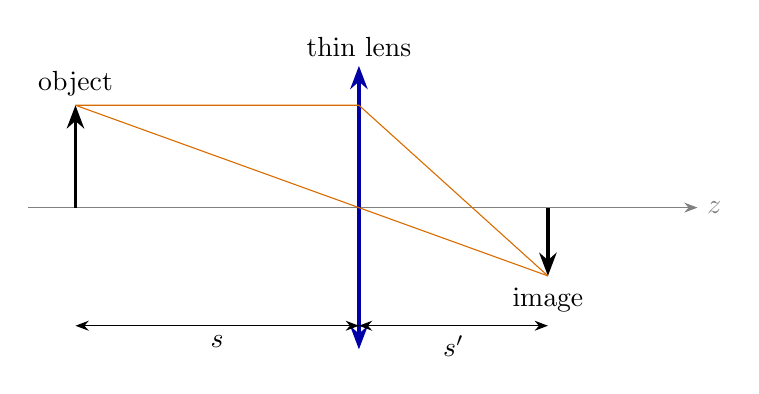
\begin{tikzpicture}[x=1cm,y=1cm,>=Stealth]
\draw[gray,->] (-4.2,0)--(4.3,0) node[right] {$z$};
\draw[very thick,blue!65!black,<->] (0,-1.8)--(0,1.8);
\draw[very thick,->] (-3.6,0)--(-3.6,1.3);
\draw[very thick,->] (2.4,0)--(2.4,-0.867);
\draw[orange!85!black] (-3.6,1.3)--(0,1.3)--(2.4,-0.867);
\draw[orange!85!black] (-3.6,1.3)--(2.4,-0.867);
\node[above] at (-3.6,1.3) {object};
\node[below] at (2.4,-0.9) {image};
\node[above] at (0,1.8) {thin lens};
\draw[<->] (-3.6,-1.5)--(0,-1.5) node[midway,below] {$s$};
\draw[<->] (0,-1.5)--(2.4,-1.5) node[midway,below] {$s'$};
\end{tikzpicture}
\caption{Paraxial imaging of an off-axis point. The drawing illustrates the construction; the numerical conjugates in the worked example differ from the schematic scale.}
\end{figure}

\section{A concave spherical mirror and the origin of its focal length}
Choose the mirror vertex at $z=0$, incident light travelling in $-z$, and a concave bowl $z=s(r)=R-\sqrt{R^2-r^2}$ opening toward $+z$. For small $r$, $s'(r)\simeq r/R$. In a meridional section a unit normal is approximately $(-r/R,0,1)$. Apply Eq.~\eqref{fnd:reflection} to $\bm{d}=(0,0,-1)$: the outgoing direction is approximately $(-2r/R,0,1)$. At distance $f$ along $+z$, the transverse height is approximately $r-2fr/R$. Hence
\begin{equation}
\boxed{f=R/2.}
\label{fnd:mirrorf}
\end{equation}
For finite real object and image distances $s,s'>0$ in front of this mirror, the geometric path through surface point $r$ is
\[
\sqrt{r^2+[s-s(r)]^2}+\sqrt{r^2+[s'-s(r)]^2}.
\]
To quadratic order this is
\[
s+s'+r^2\left(\frac{1}{2s}+\frac{1}{2s'}-\frac1R\right)+O(r^4).
\]
Stationarity for all paraxial heights requires $1/s+1/s'=2/R=1/f$. The omitted quartic terms explain why a spherical mirror's finite-aperture rays generally fail to meet at one point. A paraboloid is exactly stigmatic for an on-axis collimated input under ideal specular geometric reflection; it is not generally perfect for other conjugates or off-axis fields.

\section{Translation, refraction, and a thick lens}
Use ray vector $(y,p)^{\mathsf T}$ with $p=nu$. Translation by physical distance $d$ in constant index $n$ gives $y'=y+du=y+(d/n)p$ and preserves $p$. Refraction preserves the surface intersection height and changes $p$ by $-\Phi y$. The matrices are therefore
\begin{equation}
T(d,n)=\begin{pmatrix}1&d/n\\0&1\end{pmatrix},\qquad
S(\Phi)=\begin{pmatrix}1&0\\-\Phi&1\end{pmatrix}.
\label{fnd:matrices}
\end{equation}
For a lens of centre thickness $d$, internal index $n_g$, and surface powers $\Phi_1,\Phi_2$,
\begin{align}
M&=S(\Phi_2)T(d,n_g)S(\Phi_1)\\
&=\begin{pmatrix}
1-d\Phi_1/n_g&d/n_g\\
-\Phi_1-\Phi_2+d\Phi_1\Phi_2/n_g&1-d\Phi_2/n_g
\end{pmatrix}
=\begin{pmatrix}A&B\\C&D\end{pmatrix}.
\end{align}
The effective power is $\Phi_{\rm eff}=-C=\Phi_1+\Phi_2-d\Phi_1\Phi_2/n_g$. In output air the effective focal length is $f_{\rm eff}=1/\Phi_{\rm eff}$. A collimated input $(y_0,0)$ emerges as $(Ay_0,Cy_0)$. Translation by a distance $b$ to the axis requires $Ay_0+bCy_0=0$, giving the back focal length measured from the second vertex:
\begin{equation}
\boxed{\mathrm{BFL}=-A/C.}
\label{fnd:bfl}
\end{equation}
Effective focal length is measured from a principal plane, an equivalent reference plane of the first-order system. Back focal length is measured from the last physical vertex. They are equal for an ideal thin lens in air but not for a general thick lens.

\paragraph{Worked thick-lens calculation.}
Retain $R_1=+50\ \mathrm{mm}$, $R_2=-50\ \mathrm{mm}$ and $n_g=1.5$, but use $d=5\ \mathrm{mm}$. Then $\Phi_1=\Phi_2=0.01\ \mathrm{mm}^{-1}$ and
\[
A=D=\frac{29}{30},\quad B=\frac{10}{3}\ \mathrm{mm},\quad
C=-\frac{59}{3000}\ \mathrm{mm}^{-1}.
\]
Consequently,
\[
f_{\rm eff}=\frac{3000}{59}=50.84746\ \mathrm{mm},\qquad
\mathrm{BFL}=\frac{2900}{59}=49.15254\ \mathrm{mm}.
\]
The paraxial focus is at global $z=5+49.15254=54.15254\ \mathrm{mm}$ if the first vertex is $z=0$. A trace reporting a different finite-height axis crossing need not be wrong: spherical aberration shifts nonparaxial rays. Compare the trace as its entrance height tends to zero before diagnosing a discrepancy.

\section{An imaging condition and a conservation check}
Include all translations from object plane to image plane in a total matrix $M$. Then $y_i=Ay_o+Bp_o$. Rays from the same object point have fixed $y_o$ but different $p_o$. They form a paraxial image when $B=0$, making $y_i=Ay_o$ independent of the launch direction.

Both matrices in Eq.~\eqref{fnd:matrices} have determinant one, so their product satisfies $AD-BC=1$. For two paraxial rays with coordinates $(y_1,p_1)$ and $(y_2,p_2)$, the combination $y_1p_2-y_2p_1$ is unchanged by such a matrix. This follows by substitution and cancellation, leaving a factor $AD-BC$. This invariant is a useful error check and is related to the restrictions on trading image size against angular spread.

\chapter{Pupils, reference wavefronts, and the meaning of an error}
\label{fnd:wavefronts}
\section{Aperture stop, entrance pupil, and exit pupil}
The \emph{aperture stop} is the element that limits the angular cone accepted from an axial object point. Its opening may be a diaphragm, a mirror boundary, or a lens rim. The \emph{entrance pupil} is the image of that stop through the optics preceding it, as seen from object space. The \emph{exit pupil} is its image through the optics following it, as seen from image space. Either image can be virtual.

These definitions explain why the pupil diameter is not always the diameter of the first lens. A stop seen through preceding optics can appear magnified. A field stop instead limits which object positions are admitted. \emph{Vignetting} occurs when off-axis bundles are partly blocked; it changes pupil shape and weights as a function of field.

The \emph{chief ray} from a field point passes through the centre of the aperture stop. A \emph{marginal ray} passes through its edge; in a centred system an axial marginal ray describes the aperture cone. Field position describes which object point is being imaged. Pupil position describes which ray from that object point is used. The two must be varied independently to characterize aberrations across an image.

For an object at infinity in air, the $f$-number is $N=f_{\rm eff}/D_{\rm entrance}$. Image-space numerical aperture is $\mathrm{NA}=n'\sin\alpha$, where $\alpha$ is the marginal cone half-angle at the image. In a simple paraxial air system with the pupil appropriately located, $\mathrm{NA}\simeq1/(2N)$. Finite conjugates, pupil magnification, and high aperture require the actual cone geometry rather than this shortcut.

\section{Define the ideal before subtracting it}
Let an output plane be $z=z_e$, with intended focus $F=(X_0,Y_0,z_f)$ and $L=z_f-z_e>0$ in a homogeneous output index $n'$. The ideal converging eikonal on that plane can be written
\begin{equation}
S_{\rm ideal}(x,y)=C-n'\sqrt{(x-X_0)^2+(y-Y_0)^2+L^2}.
\label{fnd:ideal-eikonal}
\end{equation}
The minus sign is physically necessary: the ideal transverse derivative directs a ray toward the focus. Define the optical path difference by
\begin{equation}
\boxed{W(x,y)=S_{\rm actual}(x,y)-S_{\rm ideal}(x,y).}
\label{fnd:w-sign}
\end{equation}
A positive $W$ is a positive excess of eikonal, in length units, at the same evaluation point. The choice of $C$ changes only a constant term called piston. We usually choose it so a chief-ray reference or the pupil mean is zero.

An equivalent computational construction is
\[
W=S_{\rm actual}(P)+n'|F-P|-C.
\]
The last straight distance is the distance from the evaluation point to the \emph{chosen ideal focus}. An aberrated physical ray need not travel along that line. The expression subtracts an ideal phase; it must not be described as proving that every physical ray reaches $F$.

Evaluation on a mirror surface, on a plane, or on a reference sphere gives different coordinate parameterizations. At leading order they often agree well; at higher order the mapping matters. A mode fitted as a function of mirror footprint radius is not automatically the same mode fitted over a planar exit pupil. Record the coordinate surface along with the coefficient table.

\section{Piston, tilt, and defocus}
Adding a constant $C_0$ to $W$ changes the common phase but not relative phase across a single pupil. This is \emph{piston}. It is irrelevant to the intensity of an isolated coherent image, although differential piston between interferometer arms or mirror segments can matter.

A linear wavefront $W=b_xx+b_yy$ is \emph{tilt}. Its gradient is constant, so it produces a uniform angular change in the paraxial approximation. Tilt shifts an image. Whether it should be removed depends on the question: centring a spot and predicting absolute pointing or distortion are different measurements.

A quadratic radial term is \emph{defocus}. Its connection to changing the reference image plane follows directly from Eq.~\eqref{fnd:ideal-eikonal}. For an on-axis focus,
\[
S_{\rm ideal}(r;L)=\text{piston}-\frac{n'r^2}{2L}
+\frac{n'r^4}{8L^3}-\cdots.
\]
Move the reference focus downstream by $\Delta L$, hold the actual eikonal fixed, and expand $1/(L+\Delta L)\simeq1/L-\Delta L/L^2$. The new difference is
\begin{equation}
W_{\rm new}(r)=W_{\rm old}(r)
-\frac{n'\Delta L}{2L^2}r^2
+\text{piston}+\text{higher-order terms}.
\label{fnd:reference-focus-shift}
\end{equation}
Changing the reference focus is therefore not the same operation as adding a positive quadratic phase to the physical wavefront. One changes the subtracted ideal; the other changes the actual optical system.

For normalized radius $\rho=r/a$, a quadratic coefficient $B$ in $W=B\rho^2$ changes under refocusing by $\Delta B=-n'a^2\Delta L/(2L^2)$. The units are consistent: $a^2\Delta L/L^2$ is a length.

\section{Wavefront slope to ray error: derivation and limits}
On a fixed output plane, Eq.~\eqref{fnd:eikonal} gives the exact relation between transverse direction cosines and phase:
\[
\bm{q}=(d_x,d_y)=\frac1{n'}\nabla_\perp S.
\]
Hence $\delta\bm{q}=\nabla_\perp W/n'$. If both the ideal and actual directions are paraxial, $d_z\simeq1$, so transverse slope is approximately $\bm{q}$. Propagating through axial distance $L$ yields
\begin{equation}
\boxed{\Delta\bm{x}\simeq\frac{L}{n'}\nabla_\perp W.}
\label{fnd:raygradient}
\end{equation}
The sign is positive under Eq.~\eqref{fnd:w-sign}. A positive $x$ derivative adds positive transverse direction and moves the intercept toward positive $x$. References defining ideal minus actual OPD have the opposite sign.

For a normalized wavefront $W(u,v)$ with $u=x/a$, $v=y/a$, the correct formula is $\Delta\bm{x}\simeq L\nabla_{u,v}W/(n'a)$. As an example, let $W=20\ \mathrm{nm}\,(x/a)$, $a=5\ \mathrm{mm}$, $L=100\ \mathrm{mm}$, $n'=1$. Convert $20\ \mathrm{nm}=2\times10^{-5}\ \mathrm{mm}$. Then the angle error is $4\times10^{-6}$ radians and the image shift is $0.0004\ \mathrm{mm}=0.4\ \mu\mathrm{m}$.

For higher aperture use the actual slope function on the forward branch $d_z>0$, with $|\bm{q}|<1$:
\[
\bm{s}(\bm{q})=\frac{\bm{q}}{\sqrt{1-|\bm{q}|^2}}.
\]
Let $\bm{q}_0$ be the ideal transverse direction-cosine vector at the same pupil point. Between fixed planes, exact geometrical propagation gives
\begin{equation}
\Delta\bm{x}=L\left[
\bm{s}\left(\bm{q}_0+\frac{\nabla_\perp W}{n'}\right)
-\bm{s}(\bm{q}_0)\right].
\label{fnd:exact-slope}
\end{equation}
To first order in a small wavefront perturbation, but without setting the ideal aperture angle to zero, differentiate the slope:
\[
\delta\bm{s}=
\left[\frac{I}{\sqrt{1-q_0^2}}
+\frac{\bm{q}_0\bm{q}_0^{\mathsf T}}{(1-q_0^2)^{3/2}}\right]
\frac{\nabla_\perp W}{n'}.
\]
Here $q_0^2=|\bm{q}_0|^2$ and $I$ is the two-dimensional identity matrix. This matrix approaches $I$ paraxially. Higher-order ray coefficients can receive contributions from its aperture dependence, not just from differentiating the next wavefront term. Pupil coordinate transformations and a curved evaluation surface introduce further changes. These distinctions become essential when claiming fifth-order or higher physical ray accuracy.

\section{Surface displacement is not wavefront error}
Move a local reflecting point by displacement $\delta\bm{r}$ while keeping nearby incident and outgoing reference endpoints fixed. Differentiating the lengths of the incident and outgoing segments gives
\[
\delta\mathcal{L}=n(\bm{d}_{\rm in}-\bm{d}_{\rm out})\cdot\delta\bm{r}.
\]
Let the unit normal $\bm{N}$ point toward the incident medium and let positive surface height $h$ mean displacement $h\bm{N}$. Since $\bm{d}_{\rm in}\cdot\bm{N}=-\cos i$ and $\bm{d}_{\rm out}\cdot\bm{N}=+\cos i$,
\begin{equation}
\boxed{\delta W=-2nh\cos i.}
\label{fnd:mirrorheight}
\end{equation}
At normal incidence in air the magnitude is twice the surface displacement. The sign says that moving the mirror toward the incoming beam shortens the two-way geometrical path. The relation is a first-order local perturbation with a specified normal displacement and pupil mapping. At oblique incidence a global axial sag is not the same as a normal displacement, and the footprint is distorted.

For a thin transmitted layer between fixed reference planes, replacing external material of index $n_e$ by glass of index $n_g$ through additional near-normal thickness $\delta t$ gives
\begin{equation}
\boxed{\delta W=(n_g-n_e)\delta t.}
\label{fnd:transmittedthickness}
\end{equation}
Thus $10\ \mathrm{nm}$ of local mirror height and $10\ \mathrm{nm}$ of extra glass thickness do not imply the same phase error. The surface-to-wavefront conversion also depends on the number of passes, incidence angle, refractive index, and spatial mapping. A manufacturer's ``surface RMS'' cannot be inserted into a wavefront formula without this information.

\chapter{Build an exact geometrical calculation you can inspect}
\label{fnd:exacttrace}
\section{What must be specified}
An optical prescription needs surface shapes and vertex positions, material index in each space, clear apertures, input field and wavelength, stop definition, and the evaluation plane or reference sphere. A conic constant by itself is not a mirror prescription. A list of Zernike coefficients without a pupil radius and convention is not a complete wavefront specification.

Use a single consistent length unit internally. Store the physical vacuum wavelength in the same unit when converting OPL to phase. Separate source rays, geometry, index data, and analysis choices so you can change one without silently changing the others. The introductory geometrical sequence is also developed in the university course collection listed as Ref.~\cite{greivenkamp502}; the derivations here are presented explicitly for independent study.

\section{Intersect a ray with a sphere}
For sphere centre $\bm{c}$ and radius magnitude $|R|$, substitute the ray $\bm{r}(t)=\bm{r}_0+t\bm{d}$ into $|\bm{r}-\bm{c}|^2=R^2$. Since $|\bm{d}|=1$, expansion gives
\[
t^2+2bt+c_0=0,\qquad
b=\bm{d}\cdot(\bm{r}_0-\bm{c}),\quad
c_0=|\bm{r}_0-\bm{c}|^2-R^2.
\]
The solutions are $t=-b\pm\sqrt{b^2-c_0}$. A negative discriminant means the line misses the sphere. But a positive discriminant does not tell you which solution belongs to the intended optical surface. A lens uses one cap of a sphere, not its entire boundary. Select a forward intersection consistent with the cap containing the specified vertex, then check the clear aperture. Close to a surface, exclude a zero-distance self-intersection within a stated numerical tolerance.

For numerical stability, if one root suffers subtraction of nearly equal numbers, compute the more stable root $q=-b-\operatorname{sign}(b)\sqrt{b^2-c_0}$ and the other as $c_0/q$, with suitable handling of zero $b$ or $q$. This follows because the product of the roots is $c_0$. Precision lost in a geometric intersection can corrupt a much smaller wavefront difference downstream.

\section{Intersect a ray with an asphere}
For an explicit surface $z=z_v+s(x,y)$, define
\[
F(t)=z_0+td_z-z_v-s(x_0+td_x,y_0+td_y).
\]
The intersection satisfies $F(t)=0$. Its derivative is
\[
F'(t)=d_z-s_xd_x-s_yd_y.
\]
Newton's iteration is $t_{k+1}=t_k-F(t_k)/F'(t_k)$. It comes from replacing $F$ near $t_k$ by its tangent line and finding that line's zero. Use a bracketed or safeguarded method if the derivative becomes small or several intersections are possible. A converged root must still be checked against the intended surface branch and aperture.

At the resulting point, an unnormalized surface normal is $(-s_x,-s_y,1)$. Normalize it by its Euclidean length and orient it according to the reflection or refraction convention. Surface position and surface slope enter different stages of the ray trace, which is why a small but rapidly varying height error can scatter rays strongly.

\section{Accumulate OPL and compare on a common plane}
For every straight segment of length $\ell_j$, add $n_j\ell_j$ before changing the material index at its end. For a collimated input, rays should start on a common plane of equal initial phase, or carry the correct initial eikonal for their different start positions. For a point object, the path from that object to the first intersection supplies the initial optical path.

After the last surface, propagate each physical ray to the same output plane $z=z_e$ using
\[
t_e=\frac{z_e-z_{\mathrm{last}}}{d_z},\qquad
P_e=P_{\mathrm{last}}+t_e\bm{d}.
\]
For a real downstream plane $t_e$ should be nonnegative. A virtual pupil may be represented by signed backward continuation in a homogeneous image space; this is a mathematical evaluation, not another physical pass through earlier surfaces.

Let $\mathcal{L}_j(P_e)$ be the accumulated actual eikonal at that point, including the final continuation with the appropriate sign. Choose reference focus $F$ and reference ray $c$. Then compute
\begin{equation}
W_j=\mathcal{L}_j(P_{e,j})+n'|F-P_{e,j}|
-\left[\mathcal{L}_c(P_{e,c})+n'|F-P_{e,c}|\right].
\label{fnd:trace-opd}
\end{equation}
The ray's pupil coordinates should be the coordinates used for the stated fit. If you sample uniformly on an entrance disk and fit on an exit disk, the mapped points need not be uniform in exit area. Use area weights or explicitly label the result as an entrance-pupil parameterization.

\section{A trace is not verified merely because it produces a spot}
Several independent checks test different failure modes:
\begin{enumerate}
\item Confirm $|\bm{d}|=1$ after every reflection or refraction and verify the tangential Snell relation at every transmitting surface.
\item Let an entrance ray height tend toward zero. Its focal distance should approach the paraxial matrix result.
\item For a centred rotationally symmetric on-axis system, rotate the input pupil ray and confirm that the output rotates correspondingly.
\item For an ideal paraboloid and axial plane-wave illumination, verify constant phase-to-focus over the admitted aperture.
\item Increase pupil sampling and fitted polynomial order separately. A low residual at sparse sample points is not evidence of an accurate continuous fit.
\item Verify that a fitted coefficient has the predicted aperture scaling in the small-aperture limit. A leading quartic wavefront scales as $a^4$ before normalization changes.
\end{enumerate}
An optical model can pass one check and fail another. For example, a wrong OPL accumulator can coexist with a correct ray spot because directions were traced correctly. Conversely, an apparently smooth OPD map can be assigned to the wrong pupil coordinates.

\section{Numerical differentiation and cancellation}
The centred finite difference $[W(x+h)-W(x-h)]/(2h)$ approximates $W'(x)$ with leading truncation error proportional to $h^2$ for a smooth function. Making $h$ arbitrarily small eventually amplifies floating-point noise. Check a sequence of step sizes for a stable region instead of assuming the smallest step is best.

Likewise, subtracting two OPLs of tens of millimetres to recover nanometres involves cancellation. Double precision is often adequate for the examples in these books, but it is not a universal guarantee at picometre accuracy or extreme geometric scales. Use reference-subtracted analytic expressions, compensated accumulation, or higher precision when convergence checks demand it. Test the optical quantity of interest, not just the number of printed digits.

\chapter{Foundation exercises and worked solutions}
\label{fnd:exercises}
\section{Exercises}
Attempt these before reading the solutions. State units and conventions in every answer.
\begin{enumerate}
\item A wavefront has $W=45\ \mathrm{nm}$ at one pupil point relative to another. Compute the phase difference at $633\ \mathrm{nm}$ and $13.5\ \mathrm{nm}$.
\item A spherical surface has $R=200\ \mathrm{mm}$ and clear radius $a=10\ \mathrm{mm}$. Find the quadratic sag at the edge and the first omitted quartic sag. Why can the latter matter even when the quadratic approximation looks accurate on a drawing?
\item Find the mean, RMS after removing the mean, and peak-to-valley value of $W=B\rho^4$ on a uniformly weighted unit disk.
\item A ray enters index $1.5$ from air at $30^\circ$ to the normal. Find its refracted angle. Explain why substituting $\tan i$ for $\sin i$ is not an exact refraction law.
\item Derive the focal length of a thin lens with $n_g=1.6$, $R_1=+80\ \mathrm{mm}$, $R_2=-120\ \mathrm{mm}$. Where is the image of an object $300\ \mathrm{mm}$ in front of it?
\item A normal-incidence mirror has positive normal height error $h=+8\ \mathrm{nm}$ toward the incoming beam. What is its first-order OPD in air? Compare with a transmitted glass thickness increase of $8\ \mathrm{nm}$ at $n_g=1.5$.
\item At an output plane $a=10\ \mathrm{mm}$ from its pupil centre to its edge, a reference focus lies $L=200\ \mathrm{mm}$ downstream in air. How much does the quadratic normalized-pupil coefficient change if the reference focus moves downstream by $0.1\ \mathrm{mm}$?
\item For the thick lens of Chapter~\ref{fnd:imaging}, use its matrix to find the output ray vector for collimated entrance height $1\ \mathrm{mm}$, then recover its paraxial BFL from the vector.
\item For $W=A\rho^4+B\rho^2$, choose $B$ to minimize mean-subtracted wavefront RMS. Is the resulting coefficient also guaranteed to minimize every geometrical spot measure?
\end{enumerate}

\section{Solutions with intermediate steps}
\paragraph{1. Phase.}
Use $\Delta\phi=2\pi W/\lambda_0$. At $633\ \mathrm{nm}$, $W/\lambda_0=45/633=0.071090$ and $\Delta\phi=0.44667$ radians. At $13.5\ \mathrm{nm}$ the ratio is $10/3$, so the accumulated difference is $20\pi/3=20.94395$ radians. An interference measurement of wrapped phase only determines this angle modulo $2\pi$; reconstructing a continuous multiwave OPD requires phase unwrapping or additional information.

\paragraph{2. Sag.}
The quadratic term is $a^2/(2R)=100/400=0.25\ \mathrm{mm}$. The quartic term is $a^4/(8R^3)=10^4/(8\times8\times10^6)=0.00015625\ \mathrm{mm}=156.25\ \mathrm{nm}$. It is only $0.0625\%$ of the quadratic sag, yet its normal-incidence reflected path effect has magnitude approximately $312.5\ \mathrm{nm}$ under the local perturbation model. Optical phase sensitivity and visual geometric similarity are different criteria.

\paragraph{3. Quartic statistics.}
The mean is $B\langle\rho^4\rangle=B/3$. The second moment is $B^2\langle\rho^8\rangle=B^2/5$. Therefore the variance is $B^2(1/5-1/9)=4B^2/45$ and $\sigma_W=2|B|/\sqrt{45}$. The extrema are $0$ and $B$, so peak-to-valley is $|B|$. Removing the mean leaves peak-to-valley unchanged.

\paragraph{4. Refraction.}
Snell's law gives $\sin t=\sin30^\circ/1.5=1/3$, so $t=\arcsin(1/3)=19.4712^\circ$. The sine follows from the tangential projection of a \emph{unit} direction and from the path derivative. The tangent is transverse slope per axial distance, a different geometric quantity. Sine and tangent agree to first order near zero, which explains their interchange only in a paraxial approximation.

\paragraph{5. Lens.}
The power is $0.6(1/80+1/120)=0.0125\ \mathrm{mm}^{-1}$, so $f=80\ \mathrm{mm}$. The image satisfies $1/s'=1/80-1/300=11/1200\ \mathrm{mm}^{-1}$. Thus $s'=1200/11=109.0909\ \mathrm{mm}$ and the magnification is $-s'/s=-4/11$.

\paragraph{6. Surface versus thickness.}
With the stated mirror height sign, $\delta W=-2h=-16\ \mathrm{nm}$. The transmitted thickness produces $\delta W=(1.5-1)(8\ \mathrm{nm})=+4\ \mathrm{nm}$. The signs differ because moving the reflector forward shortens the path, whereas replacing air by more glass increases optical path between fixed planes.

\paragraph{7. Reference focus.}
Equation~\eqref{fnd:reference-focus-shift} gives
\[
\Delta B=-\frac{(10\ \mathrm{mm})^2(0.1\ \mathrm{mm})}
{2(200\ \mathrm{mm})^2}=-0.000125\ \mathrm{mm}=-125\ \mathrm{nm}.
\]
The calculation assumes $|\Delta L|\ll L$ and a paraxial pupil. A physical change in lens power requires a separate calculation of how $S_{\rm actual}$ changes.

\paragraph{8. Thick-lens ray.}
Multiplication gives $y_{\mathrm{out}}=29/30\ \mathrm{mm}$ and $p_{\mathrm{out}}=-59/3000$. In output air $u\simeq p$, so the distance needed to remove the remaining height is $-y/u=(29/30)(3000/59)=2900/59\ \mathrm{mm}$. This agrees with Eq.~\eqref{fnd:bfl}. Its dimensions come from the height; reduced angle is dimensionless.

\paragraph{9. Best RMS focus.}
The variance is a quadratic function of $B$. Its derivative vanishes when
\[
0=\operatorname{Cov}(A\rho^4+B\rho^2,\rho^2)
=A\left(\frac14-\frac13\frac12\right)
+B\left(\frac13-\frac14\right)
=\frac{A+B}{12}.
\]
Therefore $B=-A$. Removing the mean yields
\[
W-\langle W\rangle=A(\rho^4-\rho^2+1/6).
\]
Squaring and using disk moments gives variance $A^2/180$. Hence $\sigma_W=|A|/\sqrt{180}$. This is best mean-square \emph{wavefront} focus under the given weighting. A geometrical metric uses derivatives or extrema and need not have the same optimum. The later chapters explicitly separate these objectives.

\part{Aberration theory: from primary terms to higher orders}
% Core chapters. Included by aberrations_textbook.tex.
% All wavefront coefficients in these chapters have dimensions of length.

\chapter{What an aberration is, and what its order means}
\label{ab:orders}

\section{The experiment behind the mathematics}
Imagine a small luminous point very far from a mirror. Cover most of the
mirror and admit a narrow pencil of rays through a small hole. Move the hole
across the mirror and record where that pencil reaches a screen. An ideal
imaging mirror sends every admitted pencil to the same image point. A real
mirror can send the pencils to different locations. The collection of their
screen intersections is a geometrical spot diagram. It describes how an
object point is spread out by geometrical optics.

There are several reasons for a spread. A sphere may have exactly its intended
shape but fail to bring a wide parallel beam to one point: that is a design
aberration. A correctly designed paraboloid may have a polishing error: that
is a fabrication error. A lens may be displaced from its intended position:
that is an alignment error. The mathematics of the emerging wavefront can
describe all three, but their remedies are different. Changing the nominal
conic constant does not repair every alignment problem; translating a detector
does not remove every polishing error.

An aberration is always measured relative to an intended mapping from object
points to image points and relative to a chosen reference wavefront. Before
reporting one, specify the object distance, field direction, wavelength,
aperture, stop position, image plane, and permitted adjustments. A statement
such as ``the spherical aberration is 50 nanometres'' is incomplete unless it
also states whether this is a polynomial coefficient, a root-mean-square
wavefront error, or a peak-to-valley error, and whether focus was removed.

\section{From exact rays to a wavefront error}
Let $\bm s$ be a unit ray direction, $n$ the refractive index, and $S$ the
eikonal, expressed as optical path length. In a homogeneous isotropic medium,
\begin{equation}
 \nabla S=n\bm s,\qquad |\nabla S|=n.
\end{equation}
The phase of a monochromatic field with vacuum wavelength $\lambda_0$ is
$2\pi S/\lambda_0$. The surfaces $S=\text{constant}$ are wavefronts; rays are
normal to them. At an interface the tangential component of $\nabla S$ is
continuous, which is the vector statement of Snell's law. At a mirror with unit
normal $\bm N$, reflection is
\begin{equation}
 \bm s_{\rm out}=\bm s_{\rm in}
       -2(\bm s_{\rm in}\cdot\bm N)\bm N.
\end{equation}
These equations are the starting point for an exact geometrical calculation.
An aberration expansion is a controlled local approximation to their result.

Choose a common output plane, use physical coordinates $\bm q=(x,y)$ on it,
and let the intended image be $\bm Q=(X,Y,L)$, where $L>0$ is the distance
forward from that plane. A converging ideal wave has eikonal
\begin{equation}
 S_{\rm id}(\bm q)=C-n'\sqrt{L^2+|\bm q-\bm Q_\perp|^2},
 \qquad \bm Q_\perp=(X,Y),
\end{equation}
where $n'$ is the image-space index and $C$ is an arbitrary common constant.
The minus sign is essential: the transverse gradient points toward the image.
Define the wavefront error by
\begin{equation}
 \boxed{W(\bm q)=S_{\rm actual}(\bm q)-S_{\rm id}(\bm q).}
 \label{ab:Wdefinition}
\end{equation}
It has units of length. A spatially constant $W$ changes the phase of the
whole pupil equally and is called piston. It does not broaden the image of
one incoherent object point.

Subtracting the two eikonal gradients gives an exact relation on this plane,
\begin{equation}
 \bm s_{\perp,\rm actual}-\bm s_{\perp,\rm id}
       =\frac{1}{n'}\nabla_{\bm q}W.
 \label{ab:directiongradient}
\end{equation}
This is a relation between \emph{direction cosines}, not directly between ray
slopes. For a forward ray,
\begin{equation}
 \bm t=\frac{\bm s_\perp}{s_z}
       =\frac{\bm s_\perp}{\sqrt{1-|\bm s_\perp|^2}},
 \qquad \bm q_{\rm image}=\bm q+L\bm t.
 \label{ab:exacttransfer}
\end{equation}
For sufficiently small angles, $s_z\simeq1$, and subtraction of the ideal
image intersection gives
\begin{equation}
 \boxed{\delta\bm q_{\rm image}\simeq
          \frac{L}{n'}\nabla_{\bm q}W.}
 \label{ab:paraxgradient}
\end{equation}
The sign is positive under definition~\eqref{ab:Wdefinition}. Books defining
the wavefront error with the opposite sign have a negative sign in this
formula. Neither convention can be used safely without its definition.

The approximation in~\eqref{ab:paraxgradient} is useful for understanding
primary aberrations. A complete fifth-order ray calculation requires more
than differentiating a sixth-degree wavefront polynomial. It also requires
the appropriate nonparaxial transfer, reference geometry, and pupil-coordinate
transformations. We will demonstrate that distinction explicitly with a
spherical mirror.

\section{Normalized aperture and field coordinates}
Let $a$ be a physical pupil radius. Write
\begin{equation}
 \bm p=(u,v)=\frac{\bm q}{a},\qquad
 \rho=\sqrt{u^2+v^2},\qquad 0\leq\rho\leq1.
\end{equation}
The polar form is $u=\rho\cos\theta$, $v=\rho\sin\theta$. Let
$\bm H=(H_x,H_y)$ denote a dimensionless object-field coordinate. For an
object at infinity, a convenient definition is
$\bm H=\bm\alpha/\alpha_{\max}$, where $\bm\alpha$ is a small field-angle
vector in radians. For a finite object, one may instead use object height
divided by a stated maximum object height. These choices produce different
numerical coefficients; neither changes the underlying physical wavefront.

Because $x=au$ and $y=av$,
\begin{equation}
 \nabla_{\bm q}W=\frac{1}{a}\nabla_{\bm p}W,
 \qquad
 \delta\bm q_{\rm image}\simeq K\nabla_{\bm p}W,
 \qquad K=\frac{L}{n'a}.
 \label{ab:K}
\end{equation}
$K$ is dimensionless. The derivative with respect to a dimensionless pupil
coordinate retains the length units of $W$, so the image displacement also
has length units. This elementary dimensional check catches many missing
pupil-radius factors.

\section{Why centered systems have an even-degree scalar expansion}
Consider a centered optical system whose surfaces are rotationally symmetric
and whose materials are isotropic. Assume it is also invariant under reflection
in a plane containing the axis, as ordinary centered mirrors and lenses are.
A simultaneous rotation or reflection of $\bm H$ and $\bm p$ must leave the
scalar optical path unchanged. Three useful invariant quantities are
\begin{equation}
 P=\bm p\cdot\bm p=u^2+v^2,\qquad
 V=\bm H\cdot\bm p=H_xu+H_yv,\qquad
 F=\bm H\cdot\bm H.
 \label{ab:invariants}
\end{equation}
Each has total degree two in the four components of field and aperture.
Every analytic scalar polynomial with these symmetries can be expressed using
these dot products. A signed two-dimensional cross product changes sign under
reflection and therefore cannot appear alone in this class of systems; its
square is already $FP-V^2$.

We can consequently organize the optical path as
\begin{equation}
 W=W_0+W_2+W_4+W_6+W_8+\cdots,
 \qquad
 W_{2k}=\sum_{i+j+\ell=k}c_{ij\ell}P^iV^jF^\ell.
 \label{ab:generalorder}
\end{equation}
The subscripts on $W_{2k}$ refer to \emph{total degree}, counting both field
and aperture. Differentiating once with respect to a pupil coordinate lowers
this degree by one. Thus a fourth-degree wavefront term produces a
third-degree ray contribution in the paraxial transfer model.

Why might one see a pupil term such as $\rho^3\cos\theta$ even though the
wavefront expansion has only even total degrees? Because its coefficient can
contain one power of field: $H\rho^3\cos\theta$ has degree four. At one fixed
nonzero field, the remaining pupil polynomial is cubic. Keeping the field
variable visible prevents this apparent contradiction.

\begin{center}
\begin{tabular}{llll}
\toprule
Wavefront degree & Leading ray degree & Typical name & Example\\
\midrule
2 & 1 & Gaussian/paraxial & $D\rho^2$\\
4 & 3 & Primary/Seidel & $S\rho^4$\\
6 & 5 & Secondary, fifth-order rays & $s\rho^6$\\
8 & 7 & Seventh-order rays & $t\rho^8$\\
\bottomrule
\end{tabular}
\end{center}

The word ``order'' also appears in Zernike analysis, where radial order $n$
specifies the highest pupil power in a particular orthogonal polynomial. For
example, primary astigmatism has a Zernike pupil polynomial of radial order
two, but its centered-system field dependence is quadratic, so its Seidel
wavefront degree is four. Primary coma has Zernike radial order three and
Seidel wavefront degree four. These are different classifications with
different purposes.

Decenter, tilt, freeform surfaces, or an asymmetric refractive-index distribution
can break the assumed symmetry. An arbitrary measured wavefront can contain
on-axis coma, trefoil, and many other terms forbidden for an ideal centered
rotationally symmetric system on axis. The absence of those terms in the
centered design model is not a claim that a manufactured system cannot have
them.

\section{Second-degree terms and the choice of reference}
At degree two there are three monomials:
\begin{equation}
 W_2=D P+M V+J F.
\end{equation}
At a fixed field, $JF$ is piston. The gradient of $MV$ is $M\bm H$, independent
of pupil position; it changes the linear image scale. The gradient of $DP$ is
$2D\bm p$, which changes convergence and therefore focus. If the reference
image has the correct Gaussian magnification and Gaussian focus, $M$ and $D$
are zero. They must be restored when a detector is displaced, or when data are
referred to an arbitrary image location.

To obtain the focus coefficient rather than memorize it, place an on-axis
ideal image at distance $L$. After removing piston,
\begin{align}
 S_{\rm id}(q;L)
 &=-n'\bigl(\sqrt{L^2+q^2}-L\bigr)\\
 &=-\frac{n'q^2}{2L}+\frac{n'q^4}{8L^3}
       -\frac{n'q^6}{16L^5}+\cdots.
\end{align}
Change the reference image to $L+\Delta z$ while holding the actual wave fixed.
To first order in $\Delta z$ and second order in pupil radius,
\begin{align}
 W_{\rm new}-W_{\rm old}
 &=-\frac{\partial S_{\rm id}}{\partial L}\Delta z\\
 &=-\frac{n'\Delta z}{2L^2}q^2+O(q^4\Delta z,\Delta z^2),
\end{align}
and hence
\begin{equation}
 \boxed{\Delta D=-\frac{n'a^2}{2L^2}\Delta z.}
 \label{ab:defocusshift}
\end{equation}
A positive downstream reference shift adds negative defocus under our
convention. The quartic and sixth-degree reference terms also change; keeping
only the quadratic term is an explicitly paraxial focus adjustment.

\chapter{Deriving and interpreting the five primary aberrations}
\label{ab:seidel}

\section{All allowed fourth-degree terms}
Degree four requires products of two invariants. There are six:
$P^2$, $PV$, $V^2$, $FP$, $FV$, and $F^2$. The last is independent of pupil
position and can be discarded when studying the image quality of a single
object point. Write the remaining five as
\begin{equation}
 \boxed{W_4=S P^2+C PV+A V^2+B FP+T FV.}
 \label{ab:W4}
\end{equation}
The letters label spherical aberration, coma, astigmatism, a field-dependent
defocus term, and distortion. They are coefficients in the particular
normalization defined above. They are not universal material constants.
Because these five monomials arise from a complete symmetry argument, this
list is complete at degree four for the stated class of systems.

Choose the field along the $u$ direction, $\bm H=(H,0)$. Then
\begin{equation}
 W_4=S(u^2+v^2)^2+CHu(u^2+v^2)
      +AH^2u^2+BH^2(u^2+v^2)+TH^3u.
 \label{ab:W4cart}
\end{equation}
The plane containing the chief ray and the optical axis is the tangential or
meridional plane; it corresponds to the $u$ direction. The perpendicular
cross-section is the sagittal direction $v$.

\section{Spherical aberration: different zones have different convergence}
Set every coefficient except $S$ to zero. Direct differentiation gives
\begin{align}
 \frac{\partial W}{\partial u}
 &=S\,2(u^2+v^2)(2u)=4Su(u^2+v^2),\\
 \frac{\partial W}{\partial v}
 &=4Sv(u^2+v^2).
\end{align}
Thus
\begin{equation}
 \delta\bm q=4KS\rho^2(u,v),\qquad
 |\delta\bm q|=4K|S|\rho^3.
 \label{ab:sphericalrays}
\end{equation}
Every annulus maps to a concentric ring at the Gaussian image plane. The
outer pupil contributes disproportionately because its transverse error grows
as the cube of radius. The pattern is rotationally symmetric and is present
on axis. The name does not imply that only spherical surfaces can produce
this aberration; a poorly chosen asphere can also produce it.

Add defocus $D\rho^2$. A meridional ray then has displacement
\begin{equation}
 \delta x=K(4Su^3+2Du).
 \label{ab:sphericalfan}
\end{equation}
A ray fan is a graph of this displacement against pupil coordinate $u$.
The cubic term curves the fan; changing focus adds a straight line. No single
straight line can cancel a nonzero cubic at every $u$. This explains why
refocusing mitigates spherical aberration without eliminating it.

To find the longitudinal displacement at which a ray from radius $q=a\rho$
crosses the axis, use its ideal slope $-q/L$ and its small aberrational slope
$4S\rho^3/(n'a)$. At a plane displaced by $\Delta z$, the leading transverse
residual is
\begin{equation}
 \delta q(\Delta z)\simeq
       \frac{4LS}{n'a}\rho^3-\frac{a\rho}{L}\Delta z.
\end{equation}
Set this to zero and solve:
\begin{equation}
 \Delta z(\rho)\simeq\frac{4L^2S}{n'a^2}\rho^2.
 \label{ab:LSA}
\end{equation}
The zero-radius limiting rays define the Gaussian focus; marginal rays have
$\rho=1$. The sign of $S$ tells which side of Gaussian focus receives the
marginal intersection under our propagation convention.

\section{Coma: an off-axis pupil ring makes a displaced image circle}
For $W=CHu(u^2+v^2)$, apply the product rule:
\begin{align}
 \frac{\partial W}{\partial u}
 &=CH\bigl[(u^2+v^2)+u(2u)\bigr]=CH(3u^2+v^2),\\
 \frac{\partial W}{\partial v}&=2CHuv.
\end{align}
Consequently,
\begin{equation}
 \delta x=KCH(3u^2+v^2),\qquad
 \delta y=2KCHuv.
 \label{ab:comarays}
\end{equation}
The displacement reverses when the field reverses. It does not reverse when
the pupil point changes from $(u,v)$ to $(-u,-v)$, since it is quadratic in
pupil coordinates. This is why opposite sides of the pupil contribute to
the same side of a comatic blur.

For a pupil ring of radius $\rho$, substitute $u=\rho\cos\theta$ and
$v=\rho\sin\theta$:
\begin{align}
 \delta x&=KCH\rho^2(2+\cos2\theta),\\
 \delta y&=KCH\rho^2\sin2\theta.
\end{align}
Let $g=KCH\rho^2$. Then
\begin{equation}
 (\delta x-2g)^2+\delta y^2=g^2.
\end{equation}
Each pupil ring therefore makes a circle of radius $|g|$ whose center is
displaced by $2g$ in the tangential direction. The union of differently sized
and displaced circles gives the characteristic comet-like distribution.
This derivation is more informative than the name because it predicts the
orientation and scaling of the spot.

For uniform pupil illumination, $\langle u^2\rangle=\langle v^2\rangle=1/4$,
so the centroid relative to the Gaussian reference is
\begin{equation}
 \langle\delta x\rangle=KCH,\qquad
 \langle\delta y\rangle=0.
\end{equation}
Removing a pupil tilt translates the whole spot; it does not erase the family
of circles. The reference point used for a spot diagram---Gaussian image,
chief-ray intersection, centroid, or diffraction maximum---must therefore be
reported.

\section{Astigmatism and the two line foci}
Retain the quadratic pupil terms, including defocus:
\begin{align}
 W&=D(u^2+v^2)+AH^2u^2+BH^2(u^2+v^2)\\
  &=D_tu^2+D_sv^2,\\
 D_t&=D+(A+B)H^2,\qquad D_s=D+BH^2.
 \label{ab:DtDs}
\end{align}
The ray displacement is
\begin{equation}
 \delta x=2KD_tu,\qquad \delta y=2KD_sv.
 \label{ab:astigrays}
\end{equation}
A pupil circle maps to an ellipse. If $D_t=0$, every tangential coordinate is
focused and the remaining image is a line in the sagittal direction. This
plane is called the \emph{tangential focus}, named for the rays that focus,
not for the orientation of the remaining line. If $D_s=0$, the remaining line
is tangential and the plane is the sagittal focus.

Use~\eqref{ab:defocusshift} to determine the two axial shifts from the current
reference plane:
\begin{equation}
 \Delta z_t=\frac{2L^2}{n'a^2}\bigl[D+(A+B)H^2\bigr],\qquad
 \Delta z_s=\frac{2L^2}{n'a^2}\bigl[D+BH^2\bigr].
 \label{ab:astigfoci}
\end{equation}
Their difference is
\begin{equation}
 \boxed{\Delta z_t-\Delta z_s=
             \frac{2L^2A}{n'a^2}H^2.}
\end{equation}
Field curvature can move both foci together; astigmatism separates them.
This distinction is observable by translating a camera through focus and
watching a spot change from one line orientation to the perpendicular one.

The midpoint of the two axial positions occurs when
\begin{equation}
 D=-\left(B+\frac{A}{2}\right)H^2.
 \label{ab:medialfocus}
\end{equation}
At that plane, $D_t=AH^2/2$ and $D_s=-AH^2/2$, giving equal-magnitude
orthogonal magnifications of the pupil. The geometrical image is a circle
for a uniformly filled circular pupil in this isolated quadratic model.
Other aberrations can make the actual best plane differ from this midpoint.

One can also see the separation algebraically from
\begin{equation}
 u^2=\frac{\rho^2}{2}\bigl(1+\cos2\theta\bigr).
\end{equation}
The Seidel term $AH^2u^2$ contains an ordinary defocus component
$AH^2\rho^2/2$ and a traceless astigmatic component
$AH^2\rho^2\cos2\theta/2$. A Zernike astigmatism polynomial contains only
the second part. Calling these two coefficient definitions identical loses a
factor of two and a field-dependent focus term.

\section{Field curvature: a sharp image surface can be curved}
When $A=0$ but $B\ne0$, the two foci coincide. Their location is
\begin{equation}
 \Delta z(H)=\frac{2L^2B}{n'a^2}H^2
\end{equation}
if the on-axis reference has $D=0$. The system can make a sharp image at each
field point, yet those points lie on a curved surface. A flat detector cannot
pass through all of them. This is an image-surface problem even when each
local point image is otherwise excellent.

If the Gaussian image height is $h'=bH$, and a shallow image surface has
sag $\Delta z=(h')^2/(2R_I)$, comparison gives
\begin{equation}
 \frac{1}{R_I}=\frac{4L^2B}{n'a^2b^2}
 \qquad(A=0).
\end{equation}
Here positive $R_I$ means the surface moves downstream with increasing
image height. When astigmatism is present, define tangential, sagittal, and
medial curvatures from~\eqref{ab:astigfoci}; they are proportional respectively
to $A+B$, $B$, and $B+A/2$. The Petzval combination is proportional to
$B-A/2$, a different quantity. These surfaces coincide only when the
astigmatism coefficient vanishes.

For a transmitted centered system with signed radii positive when their
centers of curvature lie downstream, a useful surface sum is
\begin{equation}
 \mathcal P=\sum_j\frac{n_{j+1}-n_j}{n_jn_{j+1}R_j}.
 \label{ab:petzvalsum}
\end{equation}
In an image space of index $n'$, the Petzval curvature with downstream sag
defined as above is $1/R_P=-n'\mathcal P$. Thus a positive thin lens in air
with power $\Phi$ and glass index $n$ has
$\mathcal P=\Phi/n$ and $R_P=-n/\Phi=-nf$. Its Petzval surface bends toward
the lens at increasing field height under this convention. This formula is
a paraxial centered-system result; it does not by itself predict the two
astigmatic image surfaces. A reflected system can be treated with a carefully
defined unfolded signed-index convention, but inserting mirror radii into
the transmitted formula without that convention is unsafe. Our mirror
examples use explicit reflected geometry instead.

\section{Distortion changes position without necessarily changing sharpness}
For $W=TH^3u$,
\begin{equation}
 \frac{\partial W}{\partial u}=TH^3,\qquad
 \frac{\partial W}{\partial v}=0,
\end{equation}
so every ray from this one field point receives the same displacement:
\begin{equation}
 \delta x=KTH^3,\qquad\delta y=0.
\end{equation}
An isolated distortion term does not broaden a point image. It changes the
object-to-image mapping. If the ideal image height is $bH$, then
\begin{equation}
 h'(H)=bH+KTH^3,\qquad
 \frac{h'-bH}{bH}=\frac{KT}{b}H^2.
\end{equation}
Positive and negative cubic corrections give the familiar opposite radial
distortion patterns, once the image-axis convention has been fixed.
Removing a separate tilt from every measured field wavefront hides this
information. A wavefront report with excellent residual RMS can therefore
coexist with substantial image distortion.

\section{A numerical example linking coefficients to observable errors}
Suppose $L=100\,\mathrm{mm}$, $a=10\,\mathrm{mm}$, and $n'=1$, so $K=10$.
At the maximum field $H=1$, let
\begin{equation}
 S=0.20\,\mathrm{\mu m},\quad C=0.30\,\mathrm{\mu m},\quad
 A=0.40\,\mathrm{\mu m},\quad B=-0.10\,\mathrm{\mu m},\quad
 T=0.50\,\mathrm{\mu m}.
\end{equation}
These are illustrative wavefront coefficients, not a claim about a particular
commercial lens. Spherical aberration alone produces a marginal transverse
error $4KS=8\,\mathrm{\mu m}$. Coma's outermost pupil ring has center
$2KC=6\,\mathrm{\mu m}$ and radius $KC=3\,\mathrm{\mu m}$. Distortion shifts
the entire field-point image by $KT=5\,\mathrm{\mu m}$.

For the quadratic terms, $A+B=0.30\,\mathrm{\mu m}$ and
$B=-0.10\,\mathrm{\mu m}$. Since $2L^2/a^2=200$, the tangential focus is
$60\,\mathrm{\mu m}$ downstream of the reference and the sagittal focus is
$20\,\mathrm{\mu m}$ upstream. Their separation is $80\,\mathrm{\mu m}$.
The medial focus lies $20\,\mathrm{\mu m}$ downstream. These numerical
consequences show why a list of coefficients becomes useful only after
pupil size, image distance, and reference conventions are known.

\chapter{How the aperture stop mixes aberrations}
\label{ab:stop}

\section{The stop selects rays, not merely the amount of light}
An aperture stop is the opening that limits the admitted ray bundle. Its
entrance and exit pupils are its images through the preceding and following
optics. Moving the stop can change which parts of a surface are sampled by
off-axis rays, even when all surface shapes remain unchanged. It changes
chief-ray heights and can therefore change coma, astigmatism, and distortion.

To expose the algebra, suppose a paraxial change of pupil coordinates can be
written as
\begin{equation}
 \bm p_{\rm old}=\bm p+s\bm H,
 \label{ab:stopmap}
\end{equation}
where $s$ is a dimensionless shift parameter. This simplified model keeps
the same pupil scale; a real stop change may also require rescaling, changes
of reference sphere, and vignetting analysis. It nevertheless reveals the
fundamental mixing mechanism exactly for the stated coordinate change.

The invariants transform as
\begin{equation}
 P_{\rm old}=P+2sV+s^2F,\qquad
 V_{\rm old}=V+sF,\qquad F_{\rm old}=F.
\end{equation}
For the original spherical term,
\begin{align}
 S P_{\rm old}^2
 =S\bigl[P^2+4sPV+4s^2V^2+2s^2FP
             +4s^3FV+s^4F^2\bigr].
 \label{ab:stopS}
\end{align}
Thus a quartic function of distance from one pupil center contains coma-like,
astigmatism-like, curvature-like, and distortion-like terms when expressed
about a field-shifted pupil center.

The remaining products are
\begin{align}
 V_{\rm old}P_{\rm old}
 &=VP+2sV^2+sFP+3s^2FV+s^3F^2,\\
 V_{\rm old}^2&=V^2+2sFV+s^2F^2,\\
 FP_{\rm old}&=FP+2sFV+s^2F^2,\\
 FV_{\rm old}&=FV+sF^2.
\end{align}
Collecting coefficients of the same five monomials yields
\begin{align}
 S'&=S,\\
 C'&=C+4sS,\\
 A'&=A+2sC+4s^2S,\\
 B'&=B+sC+2s^2S,\\
 T'&=T+2s(A+B)+3s^2C+4s^3S.
 \label{ab:stopcoefficients}
\end{align}
Field-only terms have again been omitted because they are piston at each
field. Notice that
\begin{equation}
 B'-\frac{A'}{2}=B-\frac{A}{2}.
\end{equation}
The cancellation is direct: $sC$ cancels half of $2sC$, and $2s^2S$ cancels
half of $4s^2S$. This is the algebraic reason the Petzval combination survives
this stop change even though the two astigmatic image surfaces change.

\section{A useful design calculation and its limitation}
If $S\ne0$, choose
\begin{equation}
 s=-\frac{C}{4S}
\end{equation}
to make $C'=0$ in the simplified model. Substitution into the astigmatism and
curvature equations gives
\begin{equation}
 A'=A-\frac{C^2}{4S},\qquad
 B'=B-\frac{C^2}{8S}.
\end{equation}
Removing coma this way generally changes other aberrations. If $S=0$, the
same pure coordinate shift leaves $C'=C$; it cannot create the missing
quartic parent term needed for this cancellation. An actual redesign can
change $S$ as well, but that is a different operation.

For example, let $S=0.10\,\mathrm{\mu m}$,
$C=0.20\,\mathrm{\mu m}$, $A=0.05\,\mathrm{\mu m}$, and
$B=0.02\,\mathrm{\mu m}$. The chosen shift is $s=-0.5$.
The new coefficients are $C'=0$, $A'=-0.05\,\mathrm{\mu m}$,
and $B'=-0.03\,\mathrm{\mu m}$. Both old and new Petzval combinations
equal $-0.005\,\mathrm{\mu m}$. A designer should now check clear apertures,
illumination, distortion, and exact off-axis rays; the algebra has identified
a tradeoff, not certified a finished optical system.

\chapter{Fifth-order rays, sixth-degree wavefronts, and beyond}
\label{ab:higher}

\section{Enumerating the complete sixth-degree invariant family}
Every sixth-degree term is a product of three members of $P,V,F$. The
number of nonnegative integer triples satisfying $i+j+\ell=3$ is
$\binom{5}{2}=10$. One triple produces $F^3$, which is field-only piston.
There are therefore nine pupil-dependent terms, not merely one ``secondary''
version of each primary aberration. Write
\begin{align}
 W_6={}&sP^3+cP^2V+ePV^2+gV^3\nonumber\\
       &+oFP^2+kFPV+a_6FV^2+b_6F^2P+t_6F^2V.
 \label{ab:W6}
\end{align}
Lowercase letters here are new independent coefficients; they are not
powers or small corrections to the uppercase coefficients in $W_4$.

For $\bm H=(H,0)$ this becomes
\begin{align}
 W_6={}&s\rho^6+cH\rho^5\cos\theta
       +eH^2\rho^4\cos^2\theta+gH^3\rho^3\cos^3\theta\nonumber\\
       &+oH^2\rho^4+kH^3\rho^3\cos\theta
       +a_6H^4\rho^2\cos^2\theta
       +b_6H^4\rho^2+t_6H^5\rho\cos\theta.
 \label{ab:W6polar}
\end{align}
The term $s\rho^6$ is sixth-degree spherical wave aberration. The $c$ term
has one power of field and five of aperture; it is often called secondary
or fifth-order aperture coma. The $o$ term has the same pupil shape as
primary spherical aberration but its amplitude grows as $H^2$. The $k$,
$a_6$, $b_6$, and $t_6$ terms increase the field dependence of primary-like
pupil patterns. Names for the $e$ and $g$ terms vary across the literature;
their explicit monomials are less ambiguous than a name.

Under the common notation $W_{hpm}$, the indices specify field power, pupil
power, and power of $\cos\theta$. Our nine terms correspond respectively to
$W_{060}$, $W_{151}$, $W_{242}$, $W_{333}$, $W_{240}$, $W_{331}$,
$W_{422}$, $W_{420}$, and $W_{511}$. This is a dictionary of polynomial
shapes only. Numerical signs and scale factors still depend on the author's
wavefront definition and pupil normalization.

\section{Deriving every fifth-degree gradient contribution}
The derivatives of the invariants follow immediately from their definitions:
\begin{equation}
 \nabla_{\bm p}P=2\bm p,\qquad
 \nabla_{\bm p}V=\bm H,\qquad
 \nabla_{\bm p}F=0.
\end{equation}
For a general monomial, the product rule therefore gives
\begin{equation}
 \nabla_{\bm p}(P^iV^jF^\ell)
 =2iP^{i-1}V^jF^\ell\bm p
  +jP^iV^{j-1}F^\ell\bm H.
 \label{ab:monomialgradient}
\end{equation}
If $i=0$ or $j=0$, omit the corresponding term; one need not interpret a
negative exponent multiplied by zero at the pupil origin.

Apply this identity to~\eqref{ab:W6}, keeping every coefficient visible:
\begin{align}
 \nabla_{\bm p}W_6={}&6sP^2\bm p
   +c(4PV\bm p+P^2\bm H)\nonumber\\
 &+e(2V^2\bm p+2PV\bm H)+3gV^2\bm H\nonumber\\
 &+4oFP\bm p+kF(2V\bm p+P\bm H)\nonumber\\
 &+2a_6FV\bm H+2b_6F^2\bm p+t_6F^2\bm H.
 \label{ab:W6gradient}
\end{align}
Every summand has total degree five. Multiplication by $K$ gives its
contribution under the paraxial wavefront-to-image transfer model.

For readers who want a directly programmable meridional and sagittal form,
put $\bm H=(H,0)$ and $P=u^2+v^2$:
\begin{align}
 \frac{\partial W_6}{\partial u}={}&
 6suP^2+cH(P^2+4u^2P)+2eH^2u(2u^2+v^2)
       +3gH^3u^2\nonumber\\
 &+4oH^2uP+kH^3(3u^2+v^2)
       +2a_6H^4u+2b_6H^4u+t_6H^5,\\
 \frac{\partial W_6}{\partial v}={}&
 6svP^2+4cHuvP+2eH^2u^2v
       +4oH^2vP+2kH^3uv+2b_6H^4v.
 \label{ab:W6cartgradient}
\end{align}
The $g$, $a_6$, and $t_6$ terms have no sagittal derivative in this coordinate
system because they depend on $u$ only. This does not make them unphysical;
the field direction has selected a preferred tangential direction.

For example, consider the mixed term
$eH^2u^2(u^2+v^2)$. It is tempting to call it simply a spherical term whose
amplitude changes with field. Differentiating shows why this is incomplete:
\begin{align}
 \frac{\partial}{\partial u}
   \bigl[eH^2(u^4+u^2v^2)\bigr]
 &=eH^2(4u^3+2uv^2),\\
 \frac{\partial}{\partial v}
   \bigl[eH^2(u^4+u^2v^2)\bigr]
 &=2eH^2u^2v.
\end{align}
At a tangential pupil point $(u,0)$ it contributes $4eH^2u^3$; at a sagittal
pupil point $(0,v)$ it contributes zero. It cannot be represented by an
isotropic quartic pupil polynomial alone.

\section{Angular harmonics explain the new shapes}
Use the trigonometric identities
\begin{equation}
 \cos^2\theta=\frac{1+\cos2\theta}{2},\qquad
 \cos^3\theta=\frac{3\cos\theta+\cos3\theta}{4}.
\end{equation}
The mixed term $eH^2\rho^4\cos^2\theta$ contains both an isotropic quartic
pupil part and a quartic astigmatic part. The term
$gH^3\rho^3\cos^3\theta$ contains both a coma-like first angular harmonic
and a trefoil-like third angular harmonic. Thus a centered system can show a
third angular harmonic at nonzero field without breaking rotational symmetry
of the \emph{whole system}: the field vector participates in that symmetry.

At one fixed field, a fit to pupil data can combine terms having the same
pupil shape. For example, the effective coefficient of $\rho^4$ includes
$S+oH^2+eH^2/2$, while the first-harmonic cubic part includes a contribution
from $C H+kH^3+3gH^3/4$. Separating these sources requires measurements or
ray traces at multiple fields. A single field's Zernike coefficients cannot
uniquely recover every field-dependent Seidel and higher-order coefficient.

\section{Why differentiating $W_6$ is not the whole fifth-order ray theory}
Let $\bm b=\bm s_{\perp,\rm id}$ and
$\bm d=\nabla_{\bm q}W/n'$. The exact transverse ray shift at the image plane is
\begin{equation}
 \delta\bm q=L\left[
    \frac{\bm b+\bm d}{\sqrt{1-|\bm b+\bm d|^2}}
   -\frac{\bm b}{\sqrt{1-|\bm b|^2}}\right].
 \label{ab:exactWray}
\end{equation}
The derivative matrix of $\bm g(\bm b)=\bm b(1-|\bm b|^2)^{-1/2}$ is
\begin{equation}
 \frac{\partial g_i}{\partial b_j}
 =\frac{\delta_{ij}}{\sqrt{1-|\bm b|^2}}
   +\frac{b_ib_j}{(1-|\bm b|^2)^{3/2}}.
\end{equation}
Expanding through second degree in the paraxial ideal direction gives
\begin{equation}
 \delta\bm q=L\left[
   \bm I+\frac{|\bm b|^2}{2}\bm I+\bm b\bm b^{\mathsf T}
   +O(|\bm b|^4)\right]\bm d+O(|\bm d|^2).
 \label{ab:transferjacobian}
\end{equation}
If $W$ begins at degree four, then $\bm d$ begins at degree three.
Multiplying that cubic contribution by the quadratic correction in brackets
produces degree five. A fifth-degree direction contribution also comes from
$\nabla W_6$. Both are required. In addition, the pupil label used for the
input ray may differ cubically from its coordinate on the common output
plane. Substituting that coordinate transformation into $W_4$ creates
sixth-degree wavefront terms. The spherical-mirror calculation below shows
all three effects without relying on a specialized surface-sum notation.

\section{The seventh-order ray family and a rule for arbitrary order}
At wavefront degree eight, the invariant exponents sum to four. The complete
pupil-dependent list is
\begin{align}
 &P^4,\quad P^3V,\quad P^2V^2,\quad PV^3,\quad V^4,\nonumber\\
 &FP^3,\quad FP^2V,\quad FPV^2,\quad FV^3,\nonumber\\
 &F^2P^2,\quad F^2PV,\quad F^2V^2,\quad F^3P,\quad F^3V.
\end{align}
There are fourteen terms. The fifteenth possible invariant, $F^4$, is piston.
Assigning an independent coefficient to each and applying
equation~\eqref{ab:monomialgradient} generates every seventh-degree pupil
gradient. For instance,
\begin{align}
 \nabla(P^2V^2)&=4PV^2\bm p+2P^2V\bm H,\\
 \nabla(FPV^2)&=F(2V^2\bm p+2PV\bm H),\\
 \nabla(F^3V)&=F^3\bm H.
\end{align}
To generate degree $2k$ systematically, loop over
$\ell=0,\ldots,k$, then $j=0,\ldots,k-\ell$, and set
$i=k-j-\ell$. Omit the one case $i=j=0$. The number of pupil-dependent
terms is
\begin{equation}
 N_{2k}=\binom{k+2}{2}-1=\frac{(k+1)(k+2)}{2}-1.
\end{equation}
This gives $2,5,9,14$ for degrees $2,4,6,8$ after field-only piston is removed.
The two degree-two terms are magnification and focus, usually incorporated
into the Gaussian reference.

This construction classifies all allowed polynomial shapes under the stated
symmetries. It does not provide the numerical coefficient of every shape for
every prescription. Those coefficients require the optical-path calculation,
a compatible higher-order surface theory, or a carefully converged exact ray
trace and fit. Calling a list of monomials a complete lens-design calculation
would confuse the basis with the solution.

\section{Scaling experiments diagnose the leading order}
Suppose an on-axis residual is dominated by a physical term $\gamma_4r^4$.
Halving the aperture radius changes its raw wavefront amplitude by $1/16$.
A physical sixth-degree term changes by $1/64$. Their paraxial transverse ray
errors scale as $a^3$ and $a^5$ respectively when image distance is unchanged.
For primary coma $W\propto\alpha r^3$, doubling the field doubles the
wavefront error; a field-cubic coma-like term increases by eight.

Performing both aperture and field scans is more informative than assigning
a name from one spot. If an alleged sixth-degree residual falls only as the
fourth power of aperture, a primary contribution remains. If it fails to
follow a clean power law at larger apertures, higher terms or vignetting may
already matter. Keep physical coefficients fixed while doing these tests:
coefficients expressed on a renormalized pupil change with $a$ by definition.

\chapter{A spherical mirror and a paraboloid, calculated from geometry}
\label{ab:mirrors}

\section{A completely specified reflected coordinate system}
Use a meridional plane $(r,z)$, with the mirror vertex at $z=0$. The reflecting
surface opens toward positive $z$; incident collimated rays travel in the
$-z$ direction and reflected rays travel toward a focus at positive $z$.
The positive number $R$ is the sphere's radius magnitude. Its sag is
\begin{equation}
 z(r)=R-\sqrt{R^2-r^2},\qquad 0\leq r<R.
 \label{ab:spheresag}
\end{equation}
This local reflected geometry is stated explicitly rather than borrowing
the transmitted-system radius signs. Set $q=\sqrt{R^2-r^2}$. A unit surface
normal is $\bm N=(-r/R,q/R)$, and the incident unit direction is $(0,-1)$.
The reflection law gives
\begin{equation}
 s_r=-\frac{2rq}{R^2},\qquad
 s_z=1-\frac{2r^2}{R^2}.
 \label{ab:mirrordirection}
\end{equation}
The subsequent forward-intercept calculation assumes $r<R/\sqrt2$, so
$s_z>0$; the asymptotic series are intended for the stronger condition
$r/R\ll1$. At $r=R/\sqrt2$ the reflected ray is parallel to the vertex
plane, and the pupil-plane extrapolation used below is singular.
For small $r/R$, the radial slope is approximately $-2r/R$. A ray starting
near $z=0$ then crosses the axis at $R/2$. Thus the paraxial focal length is
\begin{equation}f=R/2.\end{equation}

\section{Exact axial intersections and the primary ray error}
The reflected ray is
\begin{equation}
 r(t)=r+t s_r,\qquad z(t)=z(r)+t s_z.
\end{equation}
Set $r(t)=0$ to obtain $t=-r/s_r$, and substitute into $z(t)$:
\begin{align}
 z_{\rm axis}(r)
 &=z(r)-r\frac{s_z}{s_r}\\
 &=R-q+\frac{R^2-2r^2}{2q}
  =R-\frac{R^2}{2q}.
 \label{ab:sphereaxis}
\end{align}
The simplification uses $q^2=R^2-r^2$. Expand
$(1-u)^{-1/2}=1+u/2+3u^2/8+5u^3/16+\cdots$ with $u=r^2/R^2$:
\begin{equation}
 z_{\rm axis}(r)=\frac R2-\frac{r^2}{4R}
          -\frac{3r^4}{16R^3}-\frac{5r^6}{32R^5}+\cdots.
\end{equation}
Marginal rays cross closer to the mirror than paraxial rays. The leading
longitudinal spherical aberration is $-r^2/(4R)$.

At the Gaussian plane $z=f$, the exact transverse intersection is
\begin{equation}
 \epsilon(r)=r+[f-z(r)]\frac{s_r}{s_z}.
\end{equation}
Expansion gives
\begin{equation}
 \epsilon(r)=-\frac{r^3}{2R^2}-\frac{9r^5}{8R^4}
             -\frac{37r^7}{16R^6}+O(r^9/R^8).
 \label{ab:sphereexactray}
\end{equation}
The negative displacement means that the ray has already crossed the axis
when it reaches the Gaussian plane. This is an exact-reflection result; no
wavefront convention was needed to derive it.

\section{The optical-path calculation on the mirror surface}
Take a reference incoming plane at $z=z_0>z(r)$. The incident path to the
surface is $z_0-z(r)$. The distance from the surface to the intended focus
$(0,f)$ is $\sqrt{r^2+[f-z(r)]^2}$. Subtracting the axial path $z_0+f$ gives
the surface-coordinate reference-focus optical-path function
\begin{equation}
 Q(r)=n\left[-z(r)+\sqrt{r^2+[f-z(r)]^2}-f\right].
 \label{ab:surfaceQ}
\end{equation}
For an imperfect mirror the second segment is the straight segment to the
\emph{chosen reference focus}; it is generally not the actual reflected ray.
This is a generating optical-path function, not a claim that the aberrated
ray reaches that focus. Its stationary points satisfy the reflection
condition for rays that do connect to the focus.

To expand it without skipping the cancellation, write
\begin{align}
 z/R&=u/2+u^2/8+u^3/16+O(u^4),\\
 \frac{\sqrt{r^2+(f-z)^2}}{R}
 &=\sqrt{\frac54-\sqrt{1-u}}\\
 &=\frac12+\frac u2-\frac{u^2}{8}
                   +\frac{3u^3}{16}+O(u^4).
\end{align}
Subtract the sag series and the axial value $1/2$:
\begin{equation}
 \boxed{Q(r)=n\left[-\frac{r^4}{4R^3}
                    +\frac{r^6}{8R^5}+O(r^8/R^7)\right].}
 \label{ab:Qseries}
\end{equation}
The quadratic terms cancel because $f=R/2$ is the paraxial focus. A quadratic
term would remain if we chose another reference focus.

\section{Why the sixth-degree coefficient changes at an output plane}
For consistency with~\eqref{ab:Wdefinition}, describe the actual outgoing
eikonal at the common vertex plane $z=0$. Reflected rays from points with
positive sag must be extrapolated backward to this plane. This defines a
virtual pupil plane mathematically; it is not a second physical reflection.
The physical radial coordinate on that plane is
\begin{align}
 x&=r-z(r)\frac{s_r}{s_z}\\
  &=r\frac{2\sqrt{1-r^2/R^2}-1}{1-2r^2/R^2}\\
  &=r+\frac{r^3}{R^2}+\frac{7r^5}{4R^4}+O(r^7/R^6).
 \label{ab:spherepupilmap}
\end{align}
It differs from the surface footprint at cubic order. Inverting the series
by setting $r=x+\alpha x^3/R^2+\beta x^5/R^4$ gives
$\alpha=-1$ and $\beta=5/4$:
\begin{equation}
 r=x-\frac{x^3}{R^2}+\frac{5x^5}{4R^4}+O(x^7/R^6).
\end{equation}
The eikonal at the surface, after dropping a common constant, is $-nz$.
Propagation backward to $z=0$ has signed ray length $-z/s_z$, so
\begin{equation}
 S_e(x)=-nz\left(1+\frac{1}{s_z}\right).
\end{equation}
The ideal converging eikonal at that plane is
$S_{\rm id}(x)=-n[\sqrt{f^2+x^2}-f]$. Therefore
\begin{equation}
 W_e(x)=-nz\left(1+\frac1{s_z}\right)
          +n\bigl[\sqrt{f^2+x^2}-f\bigr].
\end{equation}
First expanding in $r$, and then using the inverse pupil mapping, gives
\begin{equation}
 \boxed{W_e(x)=n\left[-\frac{x^4}{4R^3}
                     +\frac{9x^6}{8R^5}+O(x^8/R^7)\right].}
 \label{ab:mirrorplaneW}
\end{equation}
The surface-coordinate function has coefficient $1/8$ at degree six;
the vertex-plane wavefront has $9/8$. The coefficient of a sixth-degree
polynomial is therefore not meaningful without the independent coordinate
and reference surface. To see the main algebraic contribution, note that
$r^4=x^4-4x^6/R^2+\cdots$: even the quartic term generates a sixth-degree
term when the pupil coordinate changes.

\section{Recovering the exact fifth-degree ray coefficient}
On the vertex plane, the ideal radial direction cosine is
\begin{equation}
 b=-\frac{x}{\sqrt{f^2+x^2}},
\end{equation}
and the exact direction perturbation is $d=W'_e(x)/n$.
In one meridional dimension, the derivative of
$g(b)=b/\sqrt{1-b^2}$ is $(1-b^2)^{-3/2}$. Hence, through fifth degree,
\begin{align}
 \epsilon(x)
 &=f\left(1+\frac{x^2}{f^2}\right)^{3/2}\frac{W'_e(x)}n+O(x^7)\\
 &=\frac R2\left(1+\frac{6x^2}{R^2}+\cdots\right)
       \left[-\frac{x^3}{R^3}+\frac{27x^5}{4R^5}+\cdots\right]\\
 &=-\frac{x^3}{2R^2}+\frac{3x^5}{8R^4}+O(x^7/R^6).
 \label{ab:mirrorfifthcheck}
\end{align}
The simple paraxial formula would give the fifth-degree coefficient $27/8$.
The direction-to-slope correction contributes $-3$, leaving $3/8$.
Finally substitute $x=r+r^3/R^2+\cdots$ into this result:
\begin{equation}
 \epsilon(r)=-\frac{r^3}{2R^2}
             +\left(-\frac32+\frac38\right)\frac{r^5}{R^4}
             +\cdots
            =-\frac{r^3}{2R^2}-\frac{9r^5}{8R^4}+\cdots,
\end{equation}
which agrees with direct reflection in~\eqref{ab:sphereexactray}. This is a
stronger check than agreement of two formulas that both made the same
paraxial approximation.

\section{An exact on-axis paraboloid needs no series cancellation}
A paraboloid with focal length $f$ has sag
\begin{equation}z(r)=\frac{r^2}{4f}.\end{equation}
Since $r^2=4fz$,
\begin{equation}
 r^2+(f-z)^2=4fz+f^2-2fz+z^2=(f+z)^2.
\end{equation}
For the physical branch $f+z>0$, the distance from the surface to the focus
is exactly $f+z$. Therefore the optical path from an incoming plane to the
focus is
\begin{equation}
 n[z_0-z+(f+z)]=n(z_0+f),
\end{equation}
independent of radius. Its derivative with respect to the surface point is
zero everywhere, which enforces reflection toward the same focus. Thus an
ideal paraboloid has no on-axis geometrical spherical aberration for a
collimated incoming beam, to any order. This statement does not assert perfect
finite-conjugate imaging or perfect off-axis imaging.

\section{Deriving the leading off-axis coma of a paraboloid}
Let the incoming direction be $(\sin\alpha,0,-\cos\alpha)$ with small
field angle $\alpha$, and let $(x,y,z)$ be a point on the paraboloid. The
incident eikonal at the surface, up to a constant, is
\begin{equation}
 S_{\rm in}=n(x\sin\alpha-z\cos\alpha).
\end{equation}
Choose the paraxial reference image $(f\alpha,0,f)$. Define a reference-focus
optical-path function by adding its distance from the surface and subtracting
the vertex value. To first order in $\alpha$,
\begin{align}
 \frac{Q_\alpha}{n}
 &=\alpha x-z+
   \sqrt{(x-f\alpha)^2+y^2+(f-z)^2}-f+O(\alpha^2)\\
 &=\alpha x-z+(f+z)-\frac{f\alpha x}{f+z}-f+O(\alpha^2)\\
 &=\alpha x\frac{z}{f+z}+O(\alpha^2)\\
 &=\frac{\alpha x(x^2+y^2)}{4f^2}
        +O(\alpha r^5/f^4,\alpha^2).
 \label{ab:parabolacoma}
\end{align}
In the square-root expansion, the first-order perturbation is
$-2f\alpha x/[2(f+z)]$. In the last line we used
$z=r^2/(4f)$ and expanded $1/(f+z)$. The leading pupil dependence is exactly
the primary-coma monomial. With $x=au$, $\alpha=\alpha_{\max}H$,
\begin{equation}
 C=\frac{n\alpha_{\max}a^3}{4f^2}
\end{equation}
for this stop-at-mirror surface-coordinate calculation to primary order.
At the pupil edge, the meridional ray displacement is approximately
$3\alpha a^2/(4f)$. For $f=500\,\mathrm{mm}$, $a=50\,\mathrm{mm}$,
and $\alpha=0.01$ radians, this is $37.5\,\mathrm{\mu m}$ relative to the
Gaussian reference. A perfect on-axis paraboloid can therefore have a
substantial off-axis blur. A complete wide-field calculation must also retain
the quadratic and higher field terms omitted in this first-order derivation.

\section{Aperture, focal ratio, and a practical numerical mirror example}
On a normalized pupil at primary order, the spherical-mirror coefficient is
\begin{equation}
 S=-\frac{na^4}{4R^3}=-\frac{na^4}{32f^3}.
\end{equation}
Take air, $R=1000\,\mathrm{mm}$, $f=500\,\mathrm{mm}$, and
$a=25\,\mathrm{mm}$. This is a $50\,\mathrm{mm}$ diameter $f/10$ mirror.
The raw quartic coefficient is $S=-97.65625\,\mathrm{nm}$. The leading
marginal longitudinal error is $-0.15625\,\mathrm{mm}$, and the leading
Gaussian-plane marginal transverse error is $-7.8125\,\mathrm{\mu m}$.
After the optimum quadratic focus and piston are removed, the primary
wavefront RMS is $|S|/\sqrt{180}=7.28\,\mathrm{nm}$, as derived in the
balancing chapter. The associated focus shift is approximately
$-0.078125\,\mathrm{mm}$.

Doubling the aperture radius to $50\,\mathrm{mm}$ while keeping $f$ fixed
multiplies the quartic coefficient and its balanced RMS by sixteen. The RMS
then becomes approximately $116.5\,\mathrm{nm}$. At $550\,\mathrm{nm}$
wavelength this is about $0.212$ waves, outside the regime where a small-error
Strehl approximation should be trusted quantitatively. The smaller mirror's
RMS is only $0.0132$ waves, for which the same approximation is well behaved.
These are geometrical design errors before adding polishing, mounting,
alignment, and environmental contributions.

\chapter{Lens aberrations: from a phase-screen model to an exact singlet}
\label{ab:lenses}

\section{What a thin optical phase screen assumes}
A thin phase screen assigns an optical-path delay to each transverse point
while ignoring the separation between the refracting surfaces. In air, a
local glass thickness $t(r)$ of index $n$ replaces the same axial thickness
of air and produces delay $(n-1)t(r)$. Removing its central piston gives
\begin{equation}
 S_{\rm screen}(r)=(n-1)[t(r)-t(0)].
 \label{ab:phasescreen}
\end{equation}
This model is especially transparent for weak phase elements and for
understanding how thickness controls phase. It is not an exact model of the
aberrations of a real curved singlet. Refraction changes ray angles inside
the glass, the path inside is oblique, and the ray reaches the second surface
at a different transverse coordinate. These effects can affect the primary
aberration coefficients themselves. Calling a lens ``thin'' in a Gaussian
power calculation does not automatically justify ignoring them in a
fourth-degree optical-path calculation.

\section{Deriving the spherical-thickness expansion}
Use transmission along $+z$. A surface vertex is at $z_j$, and its signed
radius $R_j$ is positive when its center lies downstream. Its local spherical
sag, valid on the branch through the vertex, is
\begin{equation}
 s_j(r)=\frac{r^2/R_j}{1+\sqrt{1-r^2/R_j^2}}
       =\frac{r^2}{2R_j}+\frac{r^4}{8R_j^3}
        +\frac{r^6}{16R_j^5}+O(r^8).
\end{equation}
The rationalized expression avoids a subtraction of nearly equal numbers
near $r=0$. For a lens with center thickness $t_c=z_2-z_1$,
\begin{align}
 t(r)-t_c={}&s_2(r)-s_1(r)\\
 ={}&\frac12\left(\frac1{R_2}-\frac1{R_1}\right)r^2
   +\frac18\left(\frac1{R_2^3}-\frac1{R_1^3}\right)r^4\nonumber\\
 &+\frac1{16}\left(\frac1{R_2^5}-\frac1{R_1^5}\right)r^6+\cdots.
\end{align}
The target ideal screen phase for a collimated beam focused to $f$ in air is
\begin{equation}
 S_{\rm id}(r)=-\bigl[\sqrt{f^2+r^2}-f\bigr]
       =-\frac{r^2}{2f}+\frac{r^4}{8f^3}
          -\frac{r^6}{16f^5}+\cdots.
\end{equation}
Equating the quadratic coefficients gives
\begin{equation}
 \boxed{\frac1f=(n-1)\left(\frac1{R_1}-\frac1{R_2}\right).}
\end{equation}
This is the familiar thin-lens power. It emerges here as the condition that
the quadratic wavefront error vanish.

Subtract the ideal phase from the spherical-screen phase. The fourth- and
sixth-degree physical coefficients are
\begin{align}
 \gamma_4&=\frac{n-1}{8}
       \left(\frac1{R_2^3}-\frac1{R_1^3}\right)-\frac1{8f^3},\\
 \gamma_6&=\frac{n-1}{16}
       \left(\frac1{R_2^5}-\frac1{R_1^5}\right)+\frac1{16f^5},\\
 W_{\rm screen}(r)&=\gamma_4r^4+\gamma_6r^6+\cdots.
 \label{ab:lensscreen46}
\end{align}
On a pupil of radius $a$, the dimensioned normalized coefficients are
$S=\gamma_4a^4$ and $s=\gamma_6a^6$. Their units are length even though
$\gamma_4$ has units of inverse length cubed and $\gamma_6$ inverse length
to the fifth power.

For a symmetric biconvex screen, $R_1=R$, $R_2=-R$, and
$f=R/[2(n-1)]$. With $n=1.5$, $f=R$, and
\begin{equation}
 \gamma_4=-\frac1{4R^3},\qquad \gamma_6=0.
\end{equation}
The vanishing sixth-degree coefficient does not mean that this screen is
perfect: its quartic coefficient is nonzero and its eighth-degree coefficient
is nonzero. In fact,
\begin{equation}
 W_{\rm screen}(r)=\sqrt{R^2-r^2}+\sqrt{R^2+r^2}-2R,
\end{equation}
whose terms odd in $r^2$ cancel. Taking $R=50\,\mathrm{mm}$ and
$a=5\,\mathrm{mm}$ gives $S=-1.25\,\mathrm{\mu m}$.
After primary piston and defocus balancing, the spherical Zernike coefficient
is $S/(6\sqrt5)=-0.09317\,\mathrm{\mu m}$.

An ideal phase-screen thickness could instead be chosen as
\begin{equation}
 t(r)-t(0)=-\frac{\sqrt{f^2+r^2}-f}{n-1}.
\end{equation}
This exactly supplies the desired phase in the mathematical screen model at
one wavelength. A real refracting surface must satisfy Snell's law along the
actual rays and obey thickness, slope, and material constraints. A screen
solution is consequently a useful design clue, not a finished fabrication
prescription.

\section{An exact vector-Snell algorithm for a real lens}
For a real singlet, retain the full ray state $(\bm r,\bm s)$ and accumulated
optical path $\mathcal L$. A homogeneous propagation segment of length $t$
updates them as
\begin{equation}
 \bm r_{\rm new}=\bm r+t\bm s,\qquad
 \mathcal L_{\rm new}=\mathcal L+nt.
\end{equation}
For a spherical surface with center $\bm C$ and radius magnitude $|R|$,
substitute the ray line into its equation:
\begin{align}
 |\bm r+t\bm s-\bm C|^2&=R^2,\\
 t^2+2[\bm s\cdot(\bm r-\bm C)]t
                  +|\bm r-\bm C|^2-R^2&=0.
\end{align}
Solve the quadratic and choose the forward root belonging to the intended
surface branch and aperture. A sphere has two intersections; choosing the
wrong branch can make a program produce plausible-looking but false data.

At the intersection, choose the unit normal $\bm N$ pointing into the
incident medium so that $\bm s\cdot\bm N\leq0$. Define
\begin{equation}
 \eta=\frac{n_i}{n_t},\qquad
 c_i=-\bm s\cdot\bm N,\qquad
 k_r=1-\eta^2(1-c_i^2).
\end{equation}
The transmitted direction is
\begin{equation}
 \boxed{\bm s_t=\eta\bm s+
            \left(\eta c_i-\sqrt{k_r}\right)\bm N.}
 \label{ab:vectorSnell}
\end{equation}
If $k_r<0$, there is no propagating transmitted ray in this model: total
internal reflection occurs. For $k_r\geq0$, the normal component is chosen
to point into the transmitted medium. The formula conserves the tangential
component of $n\bm s$ and produces a unit direction, providing two useful
checks on implementation.

After the last surface, propagate every ray to a common plane $z=z_e$.
For $s_z>0$, the additional distance is $(z_e-z)/s_z$. If the chosen ideal
focus is $\bm F=(0,0,z_f)$, form
\begin{equation}
 W(\bm q_e)=\mathcal L(\bm q_e)
       +n'\sqrt{(z_f-z_e)^2+|\bm q_e|^2}-\mathcal L_{\rm axial,total}.
 \label{ab:traceW}
\end{equation}
Here $\mathcal L_{\rm axial,total}$ includes the axial reference path all the
way to $z_f$. The added square-root distance defines the ideal reference
eikonal. The actual aberrated ray generally follows a different path after
the output plane. This construction therefore respects
definition~\eqref{ab:Wdefinition} without forcing the actual ray through the
reference image.

\section{A fully specified numerical biconvex singlet}
Consider a nondispersive illustrative glass with $n=1.5$, air on both sides,
front vertex $z_1=0$, rear vertex $z_2=5\,\mathrm{mm}$,
$R_1=+50\,\mathrm{mm}$, $R_2=-50\,\mathrm{mm}$, and a collimated
on-axis input beam of radius $5\,\mathrm{mm}$. These values define the
geometry and one-wavelength refractive index completely.

Use the paraxial ray vector $(y,n\theta)^{\mathsf T}$. A refracting surface
of power $\Phi_j=(n_{j+1}-n_j)/R_j$ has matrix
\begin{equation}
 \begin{pmatrix}1&0\\-\Phi_j&1\end{pmatrix},
\end{equation}
and a thickness $t$ in index $n$ has matrix
\begin{equation}
 \begin{pmatrix}1&t/n\\0&1\end{pmatrix}.
\end{equation}
For the two surfaces, both powers equal $0.01\,\mathrm{mm}^{-1}$.
Multiplying in propagation order gives
\begin{align}
 M&=\begin{pmatrix}1&0\\-0.01&1\end{pmatrix}
    \begin{pmatrix}1&5/1.5\\0&1\end{pmatrix}
    \begin{pmatrix}1&0\\-0.01&1\end{pmatrix}\\
  &=\begin{pmatrix}
   0.9666666667&3.3333333333\,\mathrm{mm}\\
   -0.0196666667\,\mathrm{mm}^{-1}&0.9666666667
   \end{pmatrix}.
\end{align}
For collimated input, the output height and angle are $Ay_0$ and $Cy_0$.
The distance from the rear vertex to the Gaussian focus is therefore
$-A/C$, not $-1/C$. The effective and back focal lengths are
\begin{equation}
 f_{\rm EFL}=-1/C=50.84745763\,\mathrm{mm},\qquad
 f_{\rm BFL}=-A/C=49.15254237\,\mathrm{mm}.
\end{equation}
Thus $z_f=54.15254237\,\mathrm{mm}$. The difference between effective and
back focal length is a principal-plane effect and is not itself an
aberration.

Now use exact intersections and~\eqref{ab:vectorSnell}, and compare
wavefronts at $z_e=6\,\mathrm{mm}$. In millimetres,
\begin{equation}
 \mathcal L_{\rm axial,total}=1.5(5)+(z_f-5).
\end{equation}
For an input ray of height $h$, its initial air path from $z=0$ to the front
surface must be included, along with the oblique glass path and final air
path to $z=6$. The table gives numerical results rounded for readability.

\begin{center}
\small
\begin{tabular}{rrrrr}
\toprule
Input $h$ & Exit height $y_e$ & Axis crossing $z$ & Spot at $z_f$ & $W(z_e)$\\
$(\mathrm{mm})$ & $(\mathrm{mm})$ & $(\mathrm{mm})$ & $(\mathrm{\mu m})$ & $(\mathrm{\mu m})$\\
\midrule
0.1 &0.0946999&54.1522301&-0.000614&-0.000000302\\
1.0 &0.9469286&54.1212944&-0.614895&-0.003020490\\
2.0 &1.8934255&54.0273484&-4.935634&-0.048357240\\
3.0 &2.8390428&53.8700924&-16.751327&-0.245055846\\
4.0 &3.7832988&53.6484893&-40.021904&-0.775586326\\
5.0 &4.7256595&53.3610500&-78.974678&-1.896913612\\
\bottomrule
\end{tabular}
\end{center}

Three observations matter. First, the marginal axial crossing is about
$0.7915\,\mathrm{mm}$ ahead of the Gaussian focus, so the real singlet
has substantial spherical aberration. Second, the raw edge wavefront error
is approximately $-1.897\,\mathrm{\mu m}$, whereas the simple spherical
screen gave $-1.25\,\mathrm{\mu m}$. Their difference is physical, not a
rounding error. Third, the output-plane coordinate $y_e$ differs from input
height $h$. A polynomial fit using $h/5$ describes the output wavefront
\emph{pulled back to entrance-ray labels}; it is not automatically an
orthogonal fit on the physical output pupil.

There is an independent differential check. At the ray with input height
$3\,\mathrm{mm}$, a numerical derivative with respect to output coordinate
gives
\begin{equation}
 \frac{dW}{dy_e}\simeq-3.4606372\times10^{-4},
\end{equation}
while exact ray directions give
\begin{equation}
 s_{y,\rm actual}-s_{y,\rm id}
       \simeq-3.4606368\times10^{-4}.
\end{equation}
Because the output is in air, these must agree by
equation~\eqref{ab:directiongradient}. Their agreement checks the optical
path, pupil coordinate, reference wavefront, and refraction calculation
together. The companion script \texttt{../verify\_optics.py} reproduces these
numbers and the spherical-mirror series.

\begin{figure}[htbp]
 \centering
 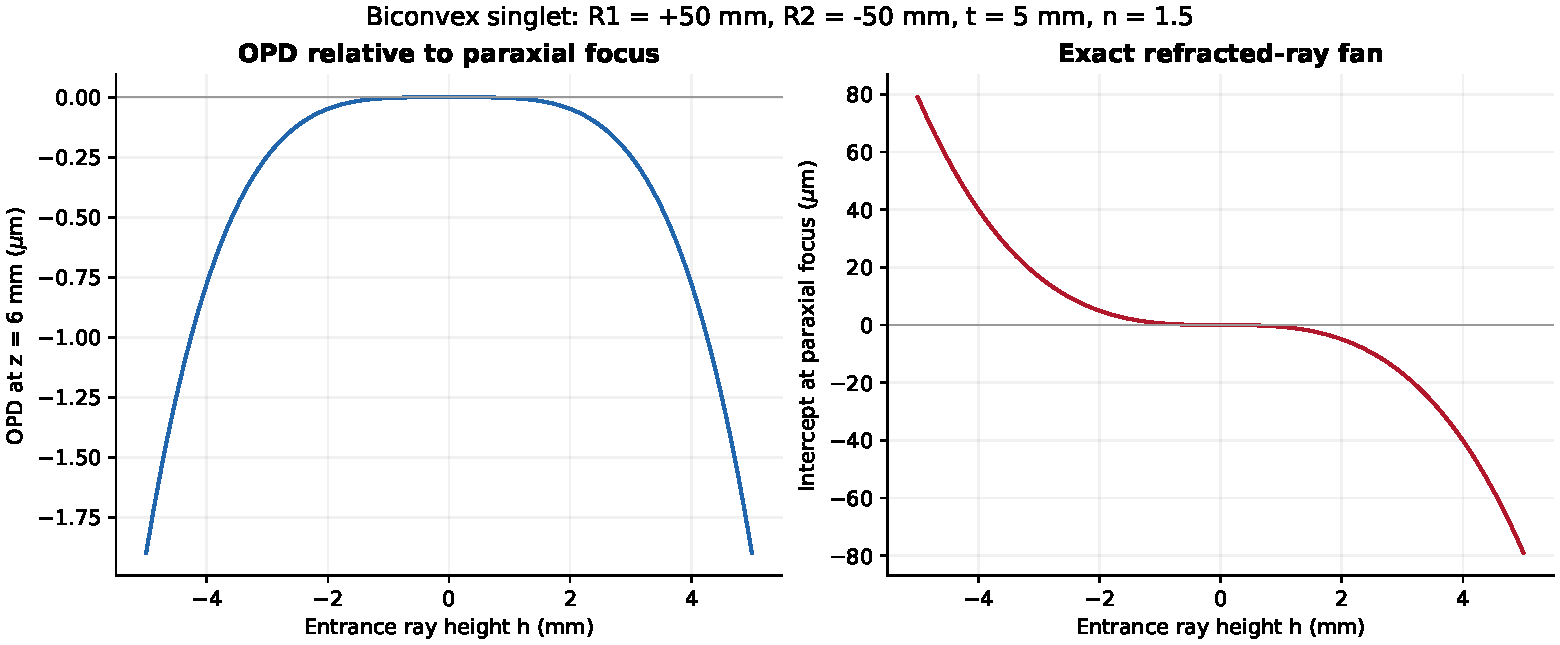
\includegraphics[width=0.95\textwidth]{../figures/thick_singlet_checks.pdf}
 \caption{The exact singlet calculation. The horizontal label uses entrance
 ray height; the wavefront itself is evaluated at the common plane
 $z=6\,\mathrm{mm}$. The ray fan shows intersections at the paraxial image
 plane. Coordinate labels are part of the definition of each plot.}
\end{figure}

\section{Changing shape, conjugates, and aspheric coefficients}
The power of a thin lens depends on the difference $1/R_1-1/R_2$. Many pairs
of radii have the same difference, hence the same paraxial focal length.
Their surface slopes and ray incidences differ, so their higher-order errors
need not agree. Changing the radii while keeping power fixed is often called
lens bending. The optimal bending also depends on object and image distance:
the ray bundle incident on a lens illuminated from infinity differs from the
bundle in a one-to-one relay.

A frequently used conic-plus-polynomial sag is
\begin{equation}
 z(r)=\frac{cr^2}{1+\sqrt{1-(1+k_c)c^2r^2}}
           +A_4r^4+A_6r^6+A_8r^8+\cdots,
 \label{ab:aspheresag}
\end{equation}
where $c=1/R$ is curvature and $k_c$ is the conic constant. Its expansion is
\begin{equation}
 z(r)=\frac{cr^2}{2}
       +\left[\frac{(1+k_c)c^3}{8}+A_4\right]r^4
       +\left[\frac{(1+k_c)^2c^5}{16}+A_6\right]r^6+\cdots.
\end{equation}
This shows explicitly why changing a conic constant changes both fourth- and
sixth-degree sag coefficients in a linked way, whereas independent $A_4$ and
$A_6$ offer separate adjustments. It also shows that a sag polynomial order
is not a wavefront aberration order: propagation, incidence, and coordinate
mapping intervene between surface height and output wavefront.

For a small normal mirror-height perturbation $h$ toward the incident medium,
the first-order local wavefront perturbation is
\begin{equation}
 \delta W=-2nh\cos i,
\end{equation}
where $i$ is the angle from the normal. A refracting surface displacement has
a corresponding first-order sensitivity containing the difference of the
incident and transmitted normal optical momenta. If the displacement is
$\delta z$ along a chosen unit normal $\bm N$, a convenient signed form is
\begin{equation}
 \delta\mathcal L=
       (n_i\bm s_i-n_t\bm s_t)\cdot\bm N\,\delta z,
\end{equation}
with incoming and outgoing endpoints held fixed. To derive it, differentiate
the lengths of the two segments: moving their common point changes the first
length by $\bm s_i\cdot\bm N\,\delta z$ and the second by
$-\bm s_t\cdot\bm N\,\delta z$. The tangential part vanishes at a stationary
ray by Snell's law. This sensitivity is useful for initial design intuition,
but a substantial shape change should be followed by an exact retrace.

\chapter{Chromatic aberration and an achromatic doublet}
\label{ab:chromatic}

\section{Wavelength is a separate variable, not a pupil order}
Geometrical reflection from a fixed ideal surface in one homogeneous medium
has wavelength-independent ray directions. Refraction depends on the ratio
of refractive indices, and these generally depend on wavelength. Thus a lens
can focus different colors at different axial positions even when each
individual monochromatic wavefront is nearly ideal. Coating phase,
diffractive elements, and wavelength-dependent media can also introduce
chromatic effects in systems containing mirrors; ``a mirror is achromatic''
is a statement about ideal geometrical reflection, not every possible
reflective instrument.

At fixed wavelength the previous polynomial classifications apply. Across a
spectrum, each coefficient can be expanded separately, for example
\begin{equation}
 S(\lambda)=S(\lambda_d)+
        \left.\frac{dS}{d\lambda}\right|_{\lambda_d}
                      (\lambda-\lambda_d)+\cdots.
\end{equation}
Wavelength variation of spherical aberration is called spherochromatism.
Correcting the Gaussian focal shift does not automatically remove it.

\section{Longitudinal color from differentiating the lens power}
For a thin lens in air, define the fixed shape factor
\begin{equation}
 G=\frac1{R_1}-\frac1{R_2},\qquad
 \Phi(\lambda)=[n(\lambda)-1]G,\qquad f(\lambda)=1/\Phi(\lambda).
\end{equation}
Differentiate $f=\Phi^{-1}$:
\begin{equation}
 \frac{df}{d\lambda}=-\frac1{\Phi^2}\frac{d\Phi}{d\lambda}
   =-f\frac1{n-1}\frac{dn}{d\lambda}.
\end{equation}
For a small index change,
\begin{equation}
 \boxed{\frac{\Delta f}{f}\simeq-\frac{\Delta n}{n-1}.}
 \label{ab:chromaticfocus}
\end{equation}
As an illustrative calculation, take $n=1.50$, $f=100\,\mathrm{mm}$,
and a blue-to-red index difference $n_F-n_C=0.010$. The blue-to-red focal
difference is approximately $f_F-f_C=-2.0\,\mathrm{mm}$. The higher-index
blue light focuses closer to a positive lens under ordinary dispersion.

For a detector fixed at the reference focus $f_d$, evaluate the wavefront
on the lens's pupil/screen plane, with pupil radius coordinate $r$ and the
detector as reference image. A wavelength whose paraxial focus is
$f_\lambda=f_d+\delta f$ then has quadratic error
\begin{equation}
 W_\lambda(r)\simeq
     \left(-\frac{1}{2f_\lambda}+\frac{1}{2f_d}\right)r^2
     \simeq\frac{\delta f}{2f_d^2}r^2.
\end{equation}
This connects longitudinal color to a wavelength-dependent defocus
coefficient. It also shows why closing the aperture reduces the wavefront
effect of a given focal mismatch even though the axial separation of the
paraxial color foci itself remains.

\section{Lateral color and the measurement convention}
For a distant object at small field angle $\alpha$, the Gaussian image height
at the best focus of each wavelength is $h'(\lambda)=f(\lambda)\alpha$.
Consequently
\begin{equation}
 \Delta h'=\alpha\Delta f,
 \qquad \frac{\Delta h'}{h'}=\frac{\Delta f}{f}.
\end{equation}
This is a wavelength-dependent image scale. In a general system, lateral
color is evaluated as a difference of image positions at a specified common
detector plane, with a stated chief-ray or centroid convention. The simple
formula above compares each color at its own Gaussian focus and must not
be silently substituted for every fixed-plane measurement.

For example, in an ideal thin-lens model with the stop exactly at the lens,
the chief ray through the center is undeviated. Its intersection with a fixed
plane can be independent of refractive power, even though the best-focus
image scale $f(\lambda)\alpha$ varies. The defocused color bundles on that
fixed plane can therefore share a chief-ray position while having different
sizes. A multi-element system with displaced pupils can behave differently.
This is another reason to define image position and plane before reporting
``lateral chromatic aberration.''

\section{Deriving the first-order achromat conditions}
For two thin lenses in contact, paraxial powers add:
\begin{equation}
 \Phi_d=\Phi_{1d}+\Phi_{2d}.
 \label{ab:achropower}
\end{equation}
For material $j$, define its Abbe number using a specified middle wavelength
$d$ and blue and red reference wavelengths $F,C$:
\begin{equation}
V_j=\frac{n_{jd}-1}{n_{jF}-n_{jC}}.
\end{equation}
For the usual visible-light $d,F,C$ convention, the reference wavelengths are
approximately $587.6\,\mathrm{nm}$, $486.1\,\mathrm{nm}$, and
$656.3\,\mathrm{nm}$ respectively. Other conventions use different spectral
lines, so retain the subscript when copying an Abbe number from a catalogue.
The surface shape factor is unchanged with wavelength, so
\begin{align}
 \Phi_{jF}-\Phi_{jC}
 &=G_j(n_{jF}-n_{jC})\\
 &=\frac{G_j(n_{jd}-1)}{V_j}
   =\frac{\Phi_{jd}}{V_j}.
\end{align}
Requiring the two selected colors to have equal total power gives
\begin{equation}
 \boxed{\frac{\Phi_{1d}}{V_1}+\frac{\Phi_{2d}}{V_2}=0.}
 \label{ab:achrocolor}
\end{equation}
Solve the two linear equations. Multiplying the color equation by $V_2$
gives $\Phi_{2d}=-(V_2/V_1)\Phi_{1d}$. Substitute into the total-power
equation and rearrange:
\begin{equation}
 \boxed{\Phi_{1d}=\Phi_d\frac{V_1}{V_1-V_2},\qquad
 \Phi_{2d}=-\Phi_d\frac{V_2}{V_1-V_2}.}
 \label{ab:achrosolution}
\end{equation}
If $V_1>V_2$ and total power is positive, the less dispersive element has
positive power and the more dispersive element negative power. If the two
Abbe numbers were equal, the denominator would vanish: two such glasses
could not provide nonzero total power and cancel this first-order color
through the contact-doublet mechanism.

\section{A worked doublet and its remaining limitations}
Choose illustrative $V_1=60$, $V_2=30$, and total focal length
$f_d=100\,\mathrm{mm}$, hence $\Phi_d=0.010\,\mathrm{mm}^{-1}$.
Equation~\eqref{ab:achrosolution} gives
\begin{equation}
 \Phi_{1d}=0.020\,\mathrm{mm}^{-1},\qquad
 \Phi_{2d}=-0.010\,\mathrm{mm}^{-1}.
\end{equation}
The individual focal lengths are $+50\,\mathrm{mm}$ and $-100\,\mathrm{mm}$.
Check the color balance explicitly:
\begin{equation}
 \frac{0.020}{60}+\frac{-0.010}{30}=0.
\end{equation}
Their individual blue-red power changes cancel while their nominal powers
sum to the required positive value.

These are first-order power allocations, not unique surface radii. They do
not determine lens bending, center thicknesses, air gaps, interface curvature,
field performance, or mechanical dimensions. They equalize two specified
colors, not an entire continuum. Differences in the detailed dispersion
curves leave secondary spectrum. If the lenses are separated by an air gap
$d$, the total thin-element power becomes
\begin{equation}
 \Phi=\Phi_1+\Phi_2-d\Phi_1\Phi_2,
\end{equation}
so the chromatic condition must also differentiate the product term.
For real glass choices, use manufacturer dispersion data or a stated
Sellmeier model, including its wavelength units and valid range. Two glasses
with similar nominal index and Abbe number need not have identical partial
dispersion. The manufacturer's technical discussion provides the data
definitions and cautions needed for that step~\cite{schottTIE29}.

\chapter{Balancing aberrations and connecting them to Zernike coefficients}
\label{ab:balance}

\section{An average over a pupil is an area average}
For a uniformly weighted full circular pupil, define
\begin{equation}
 \langle f\rangle=\frac1\pi\int_0^{2\pi}\int_0^1
        f(\rho,\theta)\rho\,d\rho\,d\theta.
 \label{ab:average}
\end{equation}
The factor $\rho$ is the polar-coordinate area element. Omitting it gives too
much weight to the center and produces incorrect optimum focus and RMS
values. For a radial power,
\begin{equation}
 \langle\rho^m\rangle=2\int_0^1\rho^{m+1}\,d\rho
          =\frac{2}{m+2}.
\end{equation}
In particular, $\langle\rho^2\rangle=1/2$,
$\langle\rho^4\rangle=1/3$, $\langle\rho^6\rangle=1/4$, and
$\langle\rho^8\rangle=1/5$. With $t=\rho^2$, the radial measure becomes
$dt$, so radial averages are especially simple integrals over $0\leq t\leq1$.

The piston-removed wavefront variance is
\begin{equation}
 \sigma_W^2=\langle(W-\langle W\rangle)^2\rangle
        =\langle W^2\rangle-\langle W\rangle^2.
\end{equation}
The RMS is its positive square root. The pupil, illumination weighting, and
removed modes are part of this definition. The results below use uniform
full-disk area weighting; a central obstruction or nonuniform weight changes
the integrals and can change the optimum focus.

\section{Deriving the least-wavefront-RMS focus for primary spherical error}
Start with $W=S\rho^4+D\rho^2+P_0$, where $D$ and piston $P_0$ may be
adjusted. Minimizing $\langle W^2\rangle$ with respect to $P_0$ gives
\begin{equation}
 \frac{\partial\langle W^2\rangle}{\partial P_0}
       =2\langle W\rangle=0,
 \qquad P_0=-S/3-D/2.
\end{equation}
After piston removal, minimizing with respect to $D$ is equivalent to
minimizing the variance of $St^2+Dt$. Its derivative is
\begin{align}
 \frac12\frac{\partial\sigma_W^2}{\partial D}
 &=S\left(\langle t^3\rangle-\langle t^2\rangle\langle t\rangle\right)
  +D\left(\langle t^2\rangle-\langle t\rangle^2\right)\\
 &=S\left(\frac14-\frac16\right)
       +D\left(\frac13-\frac14\right)=\frac{S+D}{12}.
\end{align}
The minimum therefore occurs at $D=-S$, and $P_0=S/6$. The balanced
wavefront is
\begin{equation}
 \boxed{W_{\rm bal}=S\left(\rho^4-\rho^2+\frac16\right).}
 \label{ab:balancedS}
\end{equation}
Its variance follows by direct integration:
\begin{align}
 \frac{\sigma_W^2}{S^2}
 &=\int_0^1\left(t^2-t+\frac16\right)^2dt\\
 &=\frac15-\frac12+\frac49-\frac16+\frac1{36}
  =\frac1{180}.
\end{align}
Hence
\begin{equation}
 \boxed{\sigma_W=\frac{|S|}{\sqrt{180}}.}
\end{equation}
The polynomial has equal values $S/6$ at $\rho=0$ and $\rho=1$, and value
$-S/12$ at $\rho=1/\sqrt2$. Its peak-to-valley magnitude is $|S|/4$.
RMS and peak-to-valley are therefore different numbers even for this one
simple aberration. Other shapes have different ratios.

The required detector/reference shift follows from
equation~\eqref{ab:defocusshift}: adding $D=-S$ requires
\begin{equation}
 \Delta z_{\rm wavefront}=\frac{2L^2S}{n'a^2}.
\end{equation}
It lies halfway between Gaussian focus and the leading marginal-ray focus
from~\eqref{ab:LSA}. This familiar halfway result is specific to this
aberration model and this pupil weight.

\section{Different image-quality criteria give different best focus}
For the same primary spherical model, the transverse radial displacement is
$K(4S\rho^3+2D\rho)$. Its squared geometrical RMS radius is
\begin{align}
 \sigma_r^2
 &=K^2\left\langle(4S\rho^3+2D\rho)^2\right\rangle\\
 &=K^2\left[4S^2+\frac{16}{3}SD+2D^2\right].
\end{align}
Differentiation with respect to $D$ gives
$16S/3+4D=0$, so the least-RMS-spot focus has
\begin{equation}
 D_{\rm spot}=-\frac{4S}{3},\qquad
 \sigma_{r,\min}=\frac{2K|S|}{3}.
\end{equation}
It is displaced two-thirds of the way from Gaussian to marginal-ray focus,
rather than halfway.

A third criterion minimizes the largest radius reached by any geometrical
ray, sometimes called the circle of least confusion in this model. For
$S>0$, write $D=-dS$. The normalized radial fan is
$S(4\rho^3-2d\rho)$. Its interior extremum occurs where
$12\rho^2-2d=0$. At the optimum, the positive edge excursion and negative
interior excursion have equal magnitude. Taking $d=3/2$ gives an interior
extremum at $\rho=1/2$, with value $-S$, while the edge value is $+S$.
Thus the minimum-enclosing-radius solution is
\begin{equation}
 D_{\rm enclosing}=-\frac{3S}{2},\qquad
 r_{\max,\min}=K|S|.
\end{equation}
The corresponding axial position is three-quarters of the way to marginal
focus. Reversing the sign of $S$ reverses the shifts but not these fractions.
For small aberrations, diffraction peak quality is naturally connected to
wavefront variance, not to the largest geometric ray excursion. A statement
that a calculation used ``best focus'' must name its objective.

\section{Balancing quartic and sixth-degree spherical terms together}
Let
\begin{equation}
 W=S\rho^4+s\rho^6+D\rho^2+P_0.
\end{equation}
Using $t=\rho^2$, the derivative of the piston-removed variance with respect
to $D$ contains
\begin{align}
 \operatorname{Cov}(t^2,t)&=1/12,\\
 \operatorname{Cov}(t^3,t)&=1/5-(1/4)(1/2)=3/40,\\
 \operatorname{Var}(t)&=1/12.
\end{align}
Therefore
\begin{equation}
 S/12+3s/40+D/12=0,
\end{equation}
which yields
\begin{equation}
 \boxed{D=-S-\frac9{10}s,\qquad P_0=\frac S6+\frac s5.}
 \label{ab:balance46}
\end{equation}
The second equality follows by setting
$S/3+s/4+D/2+P_0=0$. A sixth-degree error influences the optimum quadratic
focus even though it contains no explicit quadratic term before fitting.
This is one reason monomial coefficients and orthogonal coefficients differ.

If both defocus and the quartic shape are adjustable for a fixed sixth-degree
coefficient $s$, the residual can be made proportional to
\begin{equation}
 \rho^6-\frac32\rho^4+\frac35\rho^2-\frac1{20}.
\end{equation}
One obtains these numbers by demanding orthogonality to $1$, $\rho^2$, and
$\rho^4$, giving three linear integral equations. The result has RMS
$|s|/(20\sqrt7)$. This operation adjusts a fourth-degree design term as
well as focus; it is more freedom than merely translating a detector.

\section{A small Zernike dictionary with normalization made explicit}
Use real Zernike polynomials normalized to unit mean square on the full disk.
The modes needed here are
\begin{align}
 Z_0^0&=1, & Z_1^1&=2\rho\cos\theta,\\
 Z_2^0&=\sqrt3(2\rho^2-1), &
 Z_2^2&=\sqrt6\rho^2\cos2\theta,\\
 Z_3^1&=\sqrt8(3\rho^3-2\rho)\cos\theta, &
 Z_4^0&=\sqrt5(6\rho^4-6\rho^2+1),\\
 Z_6^0&=\sqrt7(20\rho^6-30\rho^4+12\rho^2-1).
\end{align}
Positive angular index denotes the cosine orientation here. Sine-oriented
modes use the same radial polynomial and normalization. No single-index
numbering convention is implied.

Solve these definitions algebraically for the monomials:
\begin{align}
 \rho^2&=\frac12+\frac{Z_2^0}{2\sqrt3},\\
 \rho^4&=\frac13+\frac{Z_2^0}{2\sqrt3}
                        +\frac{Z_4^0}{6\sqrt5},\\
 \rho^6&=\frac14+\frac{9Z_2^0}{20\sqrt3}
                   +\frac{Z_4^0}{4\sqrt5}+\frac{Z_6^0}{20\sqrt7},\\
 \rho^3\cos\theta&=\frac{Z_1^1}{3}+\frac{Z_3^1}{3\sqrt8},\\
 \rho^2\cos^2\theta&=\frac14+\frac{Z_2^0}{4\sqrt3}
                                      +\frac{Z_2^2}{2\sqrt6}.
 \label{ab:monomialZ}
\end{align}
For example, the coma identity follows from isolating $\rho^3\cos\theta$
in $Z_3^1$, then replacing $2\rho\cos\theta$ by $Z_1^1$. The result
contains both tilt and coma. An orthogonal coma mode is a \emph{balanced}
cubic pupil shape, not the raw cubic monomial.

At field $H$, after piston, both tilts, and defocus have been removed, the
primary coefficients in our orientation are
\begin{equation}
 c_4^0=\frac{S}{6\sqrt5},\qquad
 c_3^1=\frac{CH}{3\sqrt8},\qquad
 c_2^2=\frac{AH^2}{2\sqrt6}.
\end{equation}
The curvature and distortion terms enter the removed defocus and tilt
channels respectively. The remaining primary RMS is
\begin{equation}
 \boxed{\sigma_W^2=\frac{S^2}{180}
                  +\frac{C^2H^2}{72}
                  +\frac{A^2H^4}{24}.}
 \label{ab:primaryRMS}
\end{equation}
This formula assumes the modes are removed independently at the selected
field. One flat physical detector cannot independently refocus every field
point. It would therefore be inappropriate to use this locally refocused
RMS as the full-field performance of a fixed flat detector without restoring
the relevant defocus.

For quartic and sixth-degree spherical terms together,
\begin{equation}
 c_4^0=\frac{S/6+s/4}{\sqrt5},\qquad
 c_6^0=\frac{s}{20\sqrt7},
\end{equation}
and after removing piston and defocus,
\begin{equation}
 \sigma_W^2=\frac{(S/6+s/4)^2}{5}+\frac{s^2}{2800}.
\end{equation}
The term called ``sixth-degree spherical'' contributes to a fourth-radial-order
Zernike coefficient as well as to the sixth-radial-order coefficient. That
fact is not crosstalk caused by numerical error; it is the exact change of
basis. For a full explanation of arbitrary Zernike orders, fitting, and
surface-to-wavefront conversion, use the companion textbook in the
\texttt{Zernike Constants} folder.

\chapter{What diffraction adds to a ray-optics description}
\label{ab:diffraction}

\section{Rays locate geometrical energy; waves interfere}
Even an ideal aberration-free finite aperture cannot make an infinitely small
image of a point. Different parts of the pupil contribute complex amplitudes
that interfere. In scalar paraxial diffraction, an image-plane field can be
written, apart from known scale and phase factors, as
\begin{equation}
 U(\bm X)\propto\int_{\mathcal A}A(\bm q)
       \exp\left[i\frac{2\pi}{\lambda_0}W(\bm q)\right]
       \exp\left[-i\frac{2\pi n'}{\lambda_0L}
                         \bm q\cdot\bm X\right]d^2q.
 \label{ab:PSF}
\end{equation}
Here $A$ is pupil amplitude, $\mathcal A$ the transmitted pupil, and
$\bm X$ the displacement from the reference image. The point-spread function
is proportional to $|U|^2$. A phase-independent pupil mask changes diffraction
even when $W=0$; a phase error changes how the existing amplitudes add.

For a clear uniformly illuminated circular aperture, the first zero of the
ideal intensity pattern occurs at approximately
\begin{equation}
 r_{\rm Airy}=1.22\frac{\lambda_0L}{n'D}
             =0.61\frac{\lambda_0}{\mathrm{NA}},
\end{equation}
where $D=2a$ and the second form uses the paraxial image-space numerical
aperture $\mathrm{NA}\simeq n'a/L$. A geometrical spot substantially smaller
than this scale does not imply an image smaller than diffraction permits.
At high numerical aperture, vector diffraction and polarization can become
necessary, and the scalar paraxial integral must be reassessed.

\section{Deriving the small-aberration Strehl approximation}
The Strehl ratio compares an aberrated peak intensity with the ideal peak
for the same pupil amplitude and transmitted power. At the chosen reference
image and for uniform pupil amplitude, the normalized complex amplitude is
\begin{equation}
 u=\left\langle e^{i\phi}\right\rangle,
 \qquad \phi=\frac{2\pi W}{\lambda_0}.
\end{equation}
Remove piston so that $\langle\phi\rangle=0$. Expanding the exponential,
\begin{equation}
 u=1+i\langle\phi\rangle-\frac12\langle\phi^2\rangle
       +O(\phi^3)
   =1-\frac12\sigma_\phi^2+O(\phi^3).
\end{equation}
Taking squared magnitude and retaining the leading loss gives
\begin{equation}
 \mathrm{SR}\simeq1-\sigma_\phi^2
       =1-\left(\frac{2\pi\sigma_W}{\lambda_0}\right)^2.
\end{equation}
A widely used positive approximation with the same small-error expansion is
\begin{equation}
 \boxed{\mathrm{SR}\simeq
      \exp\left[-\left(\frac{2\pi\sigma_W}{\lambda_0}\right)^2\right].}
 \label{ab:strehl}
\end{equation}
It is an approximation, not an identity for every wavefront shape. It is
most useful for small residual aberrations, commonly below roughly a tenth
of a wave RMS. If the desired quantity is the \emph{maximum} image intensity,
optimize the image position and focus consistently; a large unremoved tilt
would otherwise reduce the intensity at the old origin while merely moving
an ideal spot.

Solving the exponential formula for $\mathrm{SR}=0.8$ gives
\begin{equation}
 \frac{\sigma_W}{\lambda_0}
   =\frac{\sqrt{-\ln0.8}}{2\pi}\simeq0.0752.
\end{equation}
The traditional $\lambda_0/14$ RMS guideline is a nearby convenient criterion,
not an exact universal threshold. At $\lambda_0=550\,\mathrm{nm}$ and
$\sigma_W=20\,\mathrm{nm}$, the exponential estimate is approximately
$0.949$. At large aberration, evaluate the pupil integral and determine the
actual peak, encircled energy, or modulation transfer appropriate to the
research question.

\section{Why equal RMS does not mean equal images}
The small-error peak loss depends primarily on variance, but the spatial
distribution of the lost energy depends on wavefront shape. Defocus,
astigmatism, coma, and fine-scale ripple can have equal RMS while making
different point-spread functions. High-spatial-frequency surface error may
scatter energy to large angles and be poorly represented by a short Zernike
series. Obscuration and apodization also change the ideal comparison image.
Report the residual wavefront map or sufficiently converged coefficients
together with the RMS when the image structure matters.

For incoherent imaging, the optical transfer function is the Fourier transform
of the point-spread function, normalized to unity at zero spatial frequency;
its magnitude is the modulation transfer
function. It measures how strongly different spatial frequencies are
transmitted from object to image. A spot radius, a Strehl ratio, and an MTF
value answer related but different questions. A research design should choose
the metric connected to its measurement task rather than assume one scalar
describes all performance.

\chapter{A reproducible route from a prescription to research-quality results}
\label{ab:research}

\section{Separate the physical prescription from its analysis representation}
A prescription records each surface vertex, curvature, conic constant,
polynomial coefficients, clear aperture, spacing, and refractive medium, along
with stop location and object geometry. It is the physical model. A wavefront
polynomial basis, a pupil sampling grid, and a choice of reference sphere are
analysis choices. Keeping the two separate allows the same design to be
checked by multiple methods without silently changing the optics.

Begin with the Gaussian system. Trace a paraxial marginal ray from the
on-axis object through the edge of the stop and a paraxial chief ray from an
off-axis object through the stop center. Determine focal lengths, principal
planes, entrance and exit pupils, image scale, and approximate numerical
aperture. This identifies the reference image and the ray bundles whose
aberrations will be analyzed. A system that fails its focal-length or
aperture requirement does not become acceptable merely because a refitted
wavefront has small residual RMS.

Then trace exact rays. For each field and wavelength, save the full ray
history or enough intermediate values to audit it: intersection points,
normal directions, refractive indices, outgoing directions, and accumulated
optical path. Check unit-vector norms and the tangential optical-momentum
condition at every refraction. Check that every ray passes through the
intended surface branch and clear aperture. Near caustics the outgoing field
may cease to be a single smooth function on a chosen plane; a single
polynomial wavefront chart is then insufficient.

\section{Fit optical paths using the actual sampling geometry}
Suppose sampled optical paths yield wavefront values $w_i$ at known physical
pupil points. Choose basis functions $b_j$ and form the design matrix
\begin{equation}B_{ij}=b_j(\bm p_i,\bm H_i).\end{equation}
For sample weights $\omega_i>0$, solve
\begin{equation}
 \min_{\bm c}\sum_i\omega_i\left(w_i-\sum_jB_{ij}c_j\right)^2.
 \label{ab:fit}
\end{equation}
Using QR factorization or singular-value decomposition of the weighted
matrix $\sqrt{\omega_i}B_{ij}$ avoids explicitly squaring its condition
number through normal equations. Check matrix rank and singular values;
more coefficients than independent information cannot be rescued by a
different optimizer.

If fitting centered-system invariants across field, use several radii and
azimuths in the pupil and several field magnitudes. At $H=0$, every
field-dependent column vanishes. At one fixed field, some invariant
combinations share the same pupil pattern. At pupil-edge samples only,
$P=1$, so different radial powers become indistinguishable. These are
mathematical identifiability failures, not merely a shortage of numerical
precision. Interior pupil samples and independent field values are essential.

If fitting Zernikes on a full disk, projection formulas are valid only with
the corresponding disk measure. An annular aperture, spiders, missing data,
or nonuniform weighting destroys that simple orthogonality. Solve the actual
weighted least-squares problem or construct a basis orthogonal for the actual
domain. State whether weights represent pupil area, intensity, amplitude, or
measurement uncertainty; these choices answer different questions.

Increase the fit order until both coefficient changes and residuals are
consistent with the desired accuracy. Then validate on rays not used in the
fit. A tiny residual on a poorly distributed training grid does not establish
predictive accuracy. Plot residual maps and ray fans, because a scalar norm
can hide a structured error at one edge or one field.

\section{Connect fitted coefficients back to surface changes}
Let design parameters be $\bm a=(a_1,\ldots,a_m)$ and selected optical
performance quantities be $\bm c(\bm a)$. The parameters might include a
mirror conic constant, an $A_4$ sag coefficient, lens spacing, or a detector
position. A local sensitivity matrix is
\begin{equation}
 J_{ij}=\frac{\partial c_i}{\partial a_j}
   \simeq\frac{c_i(\bm a+\delta a_j\bm e_j)
                  -c_i(\bm a-\delta a_j\bm e_j)}{2\delta a_j}.
\end{equation}
The central difference cancels the leading first-order truncation bias of a
one-sided difference. Choose $\delta a_j$ large enough to exceed numerical
noise but small enough to remain locally linear, and repeat with a nearby
step size to test stability.

For small changes,
\begin{equation}\bm c(\bm a+\Delta\bm a)\simeq\bm c(\bm a)+J\Delta\bm a.\end{equation}
A constrained least-squares step can reduce selected aberrations while
retaining focal length, clear aperture, and feasible dimensions. For example,
the merit function
\begin{equation}
 \mathcal M=\sum_{f,\lambda}w_{f\lambda}\sigma_W^2(f,\lambda)
  +w_f[f_{\rm EFL}-f_{\rm target}]^2
  +w_d[\delta h'_{\rm distortion}]^2
\end{equation}
can include both image quality and mapping requirements, provided its terms
are scaled to meaningful tolerances. After each proposed physical change,
retrace the exact system. A sensitivity matrix is local and does not justify
an arbitrarily large extrapolation.

General Seidel surface sums and complete higher-order surface-transfer
coefficients are specialized tools that can greatly accelerate this process.
This book derives the invariant structure and exact illustrative systems but
does not derive every general multi-surface Seidel sum. The primary research
paper in the reading list is an appropriate next step for a complete
sixth-order surface formulation~\cite{sas2010}. The exact tracing and fitting
route above remains a concrete way to calculate coefficients when that
formulation is not yet implemented.

\section{Tolerance budgets and covariance}
Suppose small zero-mean parameter errors $\delta\bm a$ have covariance
matrix $\Sigma_a$. Linear propagation gives
\begin{equation}
 \delta\bm c=J\delta\bm a,\qquad
 \Sigma_c=J\Sigma_aJ^{\mathsf T}.
\end{equation}
For orthonormal retained wavefront modes, the expected squared RMS contains
the trace of their covariance matrix plus the squared nominal coefficient
vector. Independent random errors can often be combined statistically,
but deterministic contributions to the same mode add algebraically before
squaring. Two surfaces each producing $10\,\mathrm{nm}$ of the same signed
spherical Zernike coefficient produce $20\,\mathrm{nm}$ together, not
$\sqrt{10^2+10^2}\,\mathrm{nm}$. Equal and opposite contributions can cancel
nominally while leaving a design sensitive to small manufacturing changes.

For a near-normal mirror with small height error, an approximate independent
surface RMS allocation follows from $\sigma_W\simeq2n\sigma_h$. A target
wavefront contribution of $20\,\mathrm{nm}$ in air suggests a
$10\,\mathrm{nm}$ height RMS allocation for that contribution, with the
same aperture and removed modes. At oblique incidence the local factor
$\cos i$ and pupil mapping must be included; at short wavelengths coating
phase and spatial-frequency-dependent scattering may also matter. A
fabrication specification must state the reference figure, usable aperture,
spatial filtering, and removed modes, not just a single height number.

\section{A minimum research record}
A result is reproducible when another person can reconstruct both the optics
and the comparison used to judge it. Record the prescription and units,
material dispersion data and temperature, object and field definitions,
aperture and stop, pupil plane and normalization, wavefront sign and reference
image, fit basis and weighting, removed modes, and numerical convergence.
Include exact ray or optical-path checks that do not reuse the same
approximation as the fitted model. Preserve the code and representative
input/output data with the derivation.

The numerical companion supplied with these textbooks checks disk
orthogonality, masked least-squares fitting, primary and sixth-degree
balancing, exact reflected-ray series, and an exact thick-lens trace. Study
one check until you can explain every variable, then modify one parameter
and predict the direction and scaling of the result before running it. That
prediction-and-check loop is a practical first research exercise.

\chapter{Worked problems and guided research projects}
\label{ab:problems}

\section{Problem 1: identify three different meanings of order}
\textbf{Problem.} A centered system has a wavefront term
$W=\gamma H^2\rho^4\cos2\theta$. Determine its total wavefront degree,
leading ray degree, pupil degree at fixed field, and the Zernike radial
orders needed to represent its pupil dependence.

\textbf{Solution.} Field contributes degree two and pupil contributes degree
four, so the total wavefront degree is six. A pupil derivative gives total
degree five in the paraxial ray relation. At fixed $H$, the pupil polynomial
has degree four. For angular harmonic two, the allowed Zernike radial
orders through four are $n=2$ and $n=4$, because $n-|m|$ must be even.
The unnormalized radial polynomial for $(n,m)=(4,2)$ is
$4\rho^4-3\rho^2$, whereas that for $(2,2)$ is $\rho^2$.
Solve
\begin{equation}
 \rho^4\cos2\theta
   =\frac14(4\rho^4-3\rho^2)\cos2\theta
       +\frac34\rho^2\cos2\theta.
\end{equation}
Both radial orders are required. The names ``fourth radial order'' and
``sixth-degree wave aberration'' are simultaneously correct because they
count different variables.

\section{Problem 2: compute three spherical-aberration focus choices}
\textbf{Problem.} An air system has $L=200\,\mathrm{mm}$,
$a=20\,\mathrm{mm}$, and primary spherical coefficient
$S=0.12\,\mathrm{\mu m}$. Find its marginal longitudinal error, least-RMS
wavefront focus shift, least-RMS spot focus shift, and balanced wavefront RMS.

\textbf{Solution.} First convert $S$ to millimetres:
$S=0.00012\,\mathrm{mm}$. The common factor is
$L^2/a^2=40000/400=100$. Therefore
\begin{align}
 \Delta z_{\rm marginal}&=4(100)(0.00012)=0.048\,\mathrm{mm},\\
 \Delta z_{\rm wavefront}&=2(100)(0.00012)=0.024\,\mathrm{mm}.
\end{align}
The least-RMS-spot focus is two-thirds of the marginal shift, or
$0.032\,\mathrm{mm}$. The minimum-enclosing-radius plane is three-quarters
of the marginal shift, or $0.036\,\mathrm{mm}$. All are downstream because
$S$ is positive in this example. The balanced RMS is
\begin{equation}
 \sigma_W=0.12/\sqrt{180}\,\mathrm{\mu m}
         =8.94\,\mathrm{nm}.
\end{equation}
Here $K=L/a=10$. At the least-RMS-spot plane, the geometrical RMS radius is
$2K|S|/3=0.80\,\mathrm{\mu m}$. This geometrical number does not replace
the diffraction calculation at the operating wavelength.

\section{Problem 3: derive the circle-of-least-confusion choice}
\textbf{Problem.} Complete the minimax derivation for a primary spherical ray
fan $4S\rho^3+2D\rho$, with $S>0$ and $0\leq\rho\leq1$.

\textbf{Solution.} Set $D=-dS$. For $0<d<2$, the edge fan value
$S(4-2d)$ is positive. The interior minimum occurs at
$\rho_* =\sqrt{d/6}$ and has value
\begin{align}
 S(4\rho_*^3-2d\rho_*)
 &=S\left(\frac{2d}{3}-2d\right)\rho_*\\
 &=-\frac{4Sd}{3}\sqrt{d/6}.
\end{align}
The edge magnitude decreases with $d$ while the interior magnitude increases.
The smallest possible larger magnitude therefore occurs where they are
equal:
\begin{equation}
 4-2d=\frac{4d}{3}\sqrt{d/6}.
\end{equation}
Substituting $d=3/2$ gives $1=1$; monotonicity makes this intersection unique
in the relevant interval. Then $\rho_*=1/2$, and both extreme magnitudes
are $S$. Multiplication by $K$ gives the minimum enclosing radius $KS$.
This argument explains the optimization criterion rather than relying on
the historical name of the focus plane.

\section{Problem 4: reconstruct a coma ring and its references}
\textbf{Problem.} At field $H=0.5$, let $C=0.24\,\mathrm{\mu m}$ and
$K=20$. Find the outer comatic ring, the centroid, and the residual RMS
after least-wavefront-RMS tilt removal.

\textbf{Solution.} The field-scaled coefficient is $CH=0.12\,\mathrm{\mu m}$.
For $\rho=1$, $g=KCH=2.4\,\mathrm{\mu m}$. The ring is
\begin{equation}
 (\delta x-4.8\,\mathrm{\mu m})^2+\delta y^2
       =(2.4\,\mathrm{\mu m})^2.
\end{equation}
The full-pupil centroid is $2.4\,\mathrm{\mu m}$ along the field direction.
Using the Zernike expansion, the unremoved tilt coefficient is
$CH/3=0.04\,\mathrm{\mu m}$ multiplying $Z_1^1=2u$.
Removing it adds a pupil ramp $-(2CH/3)u$, translating every ray by
$-2KCH/3=-1.6\,\mathrm{\mu m}$. The centroid relative to that new
wavefront reference remains $0.8\,\mathrm{\mu m}$. The reference that
removes the least-squares phase tilt is therefore not identical to the
geometrical centroid reference. The residual RMS is
\begin{equation}
 \sigma_W=|CH|/\sqrt{72}=0.01414\,\mathrm{\mu m}=14.14\,\mathrm{nm}.
\end{equation}

\section{Problem 5: choose one flat detector for two fields}
\textbf{Problem.} Ignore spherical aberration and coma. Let
$A=0.40\,\mathrm{\mu m}$ and $B=-0.10\,\mathrm{\mu m}$. For equally
weighted fields $H=0$ and $H=1$, choose the one common defocus coefficient
$D$ that minimizes mean wavefront variance after removing piston at each
field. Assume the full circular pupil and keep astigmatism.

\textbf{Solution.} The local isotropic pupil coefficient is
$D+(B+A/2)H^2=D+0.10H^2$ in micrometres. Its Zernike defocus coefficient
is this quantity divided by $2\sqrt3$. The astigmatic coefficient is
$AH^2/(2\sqrt6)$, independent of $D$, so it does not affect the derivative
with respect to the detector position. The part of the mean variance that
depends on $D$ is
\begin{equation}
 \frac12\left[\frac{D^2}{12}
                  +\frac{(D+0.10)^2}{12}\right].
\end{equation}
Differentiate: $(2D+0.10)/12=0$, hence
$D=-0.05\,\mathrm{\mu m}$. The residual Zernike defocus values are
$\mp0.05/(2\sqrt3)=\mp0.01443\,\mathrm{\mu m}$. They have equal
magnitude and opposite sign. If $L=100\,\mathrm{mm}$ and $a=10\,\mathrm{mm}$
in air, equation~\eqref{ab:defocusshift} gives a downstream detector shift
of $0.010\,\mathrm{mm}$. Independent best focus at each field would remove
both defocus values, but a single flat detector cannot realize those two
positions simultaneously.

\section{Problem 6: cancel the primary Zernike part of a sixth-degree error}
\textbf{Problem.} Suppose an adjustable system has
$W=S\rho^4+s\rho^6$ with fixed $s=0.20\,\mathrm{\mu m}$. Choose $S$
so the balanced fourth-radial-order Zernike coefficient vanishes. Find the
required added defocus and piston and the remaining RMS.

\textbf{Solution.} The fourth-order Zernike coefficient is
$(S/6+s/4)/\sqrt5$. Setting its numerator to zero gives
$S=-3s/2=-0.30\,\mathrm{\mu m}$. Then
\begin{align}
 D&=-S-0.9s=0.30-0.18=0.12\,\mathrm{\mu m},\\
 P_0&=S/6+s/5=-0.05+0.04=-0.01\,\mathrm{\mu m}.
\end{align}
The remaining wavefront is
\begin{equation}
 0.20\left(\rho^6-1.5\rho^4+0.6\rho^2-0.05\right)
       \,\mathrm{\mu m},
\end{equation}
so the only remaining radial mode through this order is
$c_6^0=0.20/(20\sqrt7)\,\mathrm{\mu m}=3.78\,\mathrm{nm}$ RMS.
The raw sixth-degree edge amplitude was $200\,\mathrm{nm}$; its much
smaller balanced RMS reflects the deliberate addition of lower-degree
shapes, not a change of units.

\section{Problem 7: identify an impossible fit before computing it}
\textbf{Problem.} A program samples only the pupil rim at one nonzero field
and attempts to fit all nine sixth-degree invariant coefficients. Explain
why this cannot work, and propose a useful sampling change.

\textbf{Solution.} On the rim, $P=1$. At one field magnitude, $F$ is also a
constant. The columns for $P^3$, $FP^2$, and $F^2P$ are therefore all
constant multiples of one another. Likewise $P^2V$, $FPV$, and $F^2V$ are
constant multiples of the same angular function. A least-squares solver
cannot distinguish coefficients whose columns are linearly dependent.
Adding more azimuths on the same rim does not fix that dependence.

Sample several distinct interior radii and several field magnitudes,
including but not limited to zero. Include pupil azimuths that distinguish
the first, second, and third angular harmonics. Build the resulting matrix
and inspect its singular values before trusting the fit. This diagnosis is
cheaper and more informative than reporting many unstable decimal places
from a rank-deficient solution.

\section{Problem 8: design a first-order achromat and check it}
\textbf{Problem.} Use illustrative materials with $V_1=70$ and $V_2=35$
to obtain a contact-doublet focal length $200\,\mathrm{mm}$. Find individual
powers and focal lengths, then state what remains unspecified.

\textbf{Solution.} Total power is $0.005\,\mathrm{mm}^{-1}$. The two powers
are
\begin{equation}
 \Phi_1=0.005\frac{70}{35}=0.010\,\mathrm{mm}^{-1},\qquad
 \Phi_2=-0.005\frac{35}{35}=-0.005\,\mathrm{mm}^{-1}.
\end{equation}
Their focal lengths are $+100\,\mathrm{mm}$ and $-200\,\mathrm{mm}$.
Check both equations:
$0.010-0.005=0.005$ and $0.010/70-0.005/35=0$.
The result does not specify actual material dispersion curves, surface
radii, thicknesses, usable aperture, stop, spherical aberration, or field
performance. Selecting those is a subsequent design problem requiring
monochromatic and polychromatic validation.

\section{Problem 9: distinguish coherent errors from a statistical budget}
\textbf{Problem.} Two deterministic mirror errors each contribute
$+12\,\mathrm{nm}$ to the same normalized spherical wavefront mode. A
third error contributes $9\,\mathrm{nm}$ to an orthogonal astigmatism mode.
Find the total RMS. Then compare with two independent zero-mean random
spherical-mode errors each having standard deviation $12\,\mathrm{nm}$.

\textbf{Solution.} Deterministic contributions to the same mode first add:
$c_S=12+12=24\,\mathrm{nm}$. The orthogonal astigmatism contributes in
quadrature, so
\begin{equation}
 \sigma_W=\sqrt{24^2+9^2}=\sqrt{657}=25.63\,\mathrm{nm}.
\end{equation}
For the independent random spherical errors, their summed coefficient has
variance $12^2+12^2=288\,\mathrm{nm}^2$. Including the fixed astigmatism,
the expected squared RMS is $288+81=369\,\mathrm{nm}^2$, whose square root
is $19.21\,\mathrm{nm}$. This is the square root of the expected squared
RMS, not necessarily the expectation of RMS itself. Positive correlation
between the two errors would add a covariance term and raise the budget.

\section{Project 1: rebuild and falsify the spherical-mirror approximation}
Begin with the exact sag, normal, and reflected direction in
Chapter~\ref{ab:mirrors}. Reproduce the axial-crossing and transverse-fan
formulas without looking at the final series. Then evaluate a range of
$a/R$ values, retaining the physical forward-reflection condition
$a<R/\sqrt2$ and concentrating initially on much smaller ratios.

For each aperture, compare exact surface-reference optical path, the
quartic approximation, and the quartic-plus-sixth approximation. Plot the
maximum absolute difference against aperture on logarithmic axes. If the
quartic truncation is working, its leading residual scales as $a^6$; the
next truncation should scale as $a^8$ while numerical roundoff is negligible.
At very small apertures, subtracting nearly equal distances can overwhelm
the tiny OPD; use a stable algebraic form or higher precision to distinguish
roundoff from failure of the optical theory.

Next repeat using the common vertex-plane coordinate. Verify that the
sixth-degree coefficient changes but the physical ray intersections do not.
A successful project report includes both coordinate definitions, the
inverse map, an exact ray check, and the numerical range over which each
truncation meets a chosen error tolerance. This turns a familiar mirror into
a serious exercise in asymptotic modeling and reproducibility.

\section{Project 2: bend a singlet while preserving its paraxial task}
Start from the exact biconvex singlet in Chapter~\ref{ab:lenses}. Choose one
surface curvature as a design variable and solve for the other so that the
\emph{thick-lens} effective focal length remains fixed at its initial value.
Keep thickness, glass, object distance, and clear aperture stated. The
thick-lens power contains a thickness-dependent product of surface powers,
so simply keeping $1/R_1-1/R_2$ fixed is insufficient for exact Gaussian
power preservation.

For each candidate shape, trace exact on-axis rays, evaluate the output
wavefront on a stated common plane, and find the permitted best focus. Plot
balanced RMS, marginal longitudinal error, and required rear clearance
against the shape variable. Reject geometries whose surfaces cross or whose
edge thickness becomes infeasible. Add two off-axis fields and inspect coma
and astigmatism before choosing a preferred shape. The lowest on-axis RMS
alone may not meet the full imaging task.

The project is complete when an independently sampled ray set confirms the
chosen candidate's performance and a small perturbation study explains how
sensitive it is to radius and spacing errors. Include a comparison with the
phase-screen approximation, stating where and why it differs.

\section{Project 3: recover a field-dependent aberration model from data}
Generate synthetic wavefront data from known $W_4+W_6$ coefficients at several
fields and pupil points. First fit noiseless data and verify exact recovery
to numerical precision. Then remove a pupil sector, introduce a central
obstruction, and add controlled measurement noise. Compare full-disk
projection, weighted least squares, and a fit that omits sixth-degree terms.

Report coefficient bias, covariance or repeated-noise variability, condition
number, and validation residuals. Identify whether an apparent primary
coefficient changes because of true field dependence, a missing basis term,
or the altered pupil measure. Finally permit one common focus adjustment
across all fields and compare it with independent per-field defocus removal.
This project connects design aberrations, metrology, and inference---three
parts of optical research that are often studied separately but interact in
every real instrument.

\chapter*{Sources and a route to further study}
\addcontentsline{toc}{chapter}{Sources and a route to further study}
The derivations and numerical examples in these chapters were written for
this textbook and checked independently where indicated. The references
below provide primary research, university teaching material, and material
data definitions for continuing study. Their sign and normalization
conventions must be compared with this book's definitions before importing
a coefficient.

Wyant and Creath's university-hosted chapter is a useful bridge between
wavefront aberration theory and optical testing~\cite{wyantcreath}.
Sasi\'an's primary paper develops a full sixth-order theory, including
propagation and pupil effects that are essential beyond primary
aberrations~\cite{sas2010}. Greivenkamp's teaching resources support the
Gaussian and geometrical foundations~\cite{greivenkamp502}. The glass
manufacturer's technical note explains the dispersion quantities required
for reproducible chromatic calculations~\cite{schottTIE29}. Read these after
reproducing the simpler exact examples here; they will then supply a deeper
framework for questions you have already learned to formulate.

\begin{thebibliography}{9}
\raggedright
\bibitem{greivenkamp502}
John E. Greivenkamp, \emph{OPTI 502: Optical Design and Instrumentation I},
University of Arizona teaching resources.
\url{https://wp.optics.arizona.edu/jgreivenkamp/classes/opti-502/}.

\bibitem{wyantcreath}
James C. Wyant and Katherine Creath,
\emph{Basic Wavefront Aberration Theory for Optical Metrology},
in \emph{Applied Optics and Optical Engineering}, Vol.~XI (1992),
university-hosted chapter/excerpt.
\url{https://wp.optics.arizona.edu/jcwyant/wp-content/uploads/sites/13/2016/08/Zernikes.pdf}.

\bibitem{sas2010}
Jos\'e Sasi\'an, ``Theory of sixth-order wave aberrations,''
\emph{Applied Optics} \textbf{49}, D69--D95 (2010).
DOI: \href{https://doi.org/10.1364/AO.49.000D69}{10.1364/AO.49.000D69}.
\url{https://wp.optics.arizona.edu/jsasian/wp-content/uploads/sites/33/2016/03/published-six-order-theory.pdf}.

\bibitem{schottTIE29}
SCHOTT Advanced Optics, \emph{TIE-29: Refractive Index and Dispersion},
version August 2023. Manufacturer technical information available through
the optical-glass downloads collection.
\url{https://www.schott.com/en-us/products/optical-glass-p1000267/downloads}.
\end{thebibliography}

\end{document}
